\documentclass[11pt,a4paper]{article}

\usepackage{fontspec}
\setmainfont{DejaVu Serif}[ItalicFont={DejaVu Serif}, ItalicFeatures={FakeSlant=0.2}, BoldItalicFont={DejaVu Serif Bold}, BoldItalicFeatures={FakeSlant=0.2}]
\setsansfont{DejaVu Sans}
\setmonofont{DejaVu Sans Mono}[Scale=0.85]
\usepackage[margin=2.1cm,headheight=14pt]{geometry}
\usepackage{graphicx}
\usepackage[table]{xcolor}
\usepackage{listings}
\usepackage[most]{tcolorbox}
\usepackage{booktabs}
\usepackage{tabularx}
\usepackage{enumitem}
\usepackage{titlesec}
\usepackage{fancyhdr}
\usepackage[hidelinks]{hyperref}
\usepackage{float}
\usepackage{caption}
\usepackage{amssymb}
\usepackage{tikz}
\usetikzlibrary{positioning,arrows.meta,fit,backgrounds,calc}
\usepackage{multicol}
\usepackage{tocloft}
\usepackage{needspace}
\usepackage{etoolbox}

\setlength{\cftbeforesecskip}{3pt}
\setlength{\cftbeforesubsecskip}{0pt}

\setlength{\cftsubsecindent}{2.2em}
\setlength{\cftsubsecnumwidth}{2.8em}
\setlength{\cftsecnumwidth}{2.2em}
\renewcommand{\cftsubsecfont}{\small}
\renewcommand{\cftsubsecpagefont}{\small}
\renewcommand{\cfttoctitlefont}{\LARGE\sffamily\bfseries\color{accent}}

\definecolor{accent}{HTML}{1F6FEB}
\definecolor{cmdbg}{HTML}{0D1117}
\definecolor{cmdfg}{HTML}{E6EDF3}
\definecolor{outbg}{HTML}{F6F8FA}
\definecolor{outframe}{HTML}{D0D7DE}
\definecolor{notebg}{HTML}{EAF2FE}
\definecolor{rowbg}{HTML}{F1F4F8}
\setlength{\aboverulesep}{0pt}
\setlength{\belowrulesep}{0pt}
\setlength{\heavyrulewidth}{1pt}
\renewcommand{\arraystretch}{1.2}
\AtBeginEnvironment{tabularx}{\rowcolors{2}{white}{rowbg}}
\newcommand{\doc}[2]{\href{https://rechefe.github.io/ipu-emulator/#1/}{\textcolor{accent}{#2}}}
\definecolor{muted}{HTML}{57606A}

\titleformat{\section}{\LARGE\sffamily\bfseries\color{accent}}{\thesection}{0.7em}{}
\titleformat{\subsection}{\large\sffamily\bfseries}{\thesubsection}{0.7em}{}
\titlespacing*{\section}{0pt}{0pt}{0.8em}
\newcommand{\sectionbreak}{\clearpage}
\setlength{\parindent}{0pt}
\setlength{\parskip}{0.55em}
\captionsetup{font={small,sf},labelfont=bf,skip=4pt}
\setlength{\textfloatsep}{8pt}

\pagestyle{fancy}
\fancyhf{}
\fancyhead[L]{\sffamily\small\color{muted}IPU Emulator --- Getting Started}
\fancyhead[R]{\sffamily\small\color{muted}\nouppercase{\leftmark}}
\fancyfoot[C]{\sffamily\small\thepage}
\renewcommand{\headrulewidth}{0.3pt}

\lstdefinestyle{shell}{
  aboveskip=0pt, belowskip=0pt,
  basicstyle=\ttfamily\small\bfseries\color{white},
  breaklines=true, columns=fullflexible, keepspaces=true,
  showstringspaces=false, upquote=true,
  postbreak=\mbox{\textcolor{muted}{$\hookrightarrow$}\space},
}
\lstdefinestyle{output}{
  aboveskip=0pt, belowskip=0pt,
  basicstyle=\ttfamily\scriptsize\color{termfg},
  breaklines=true, columns=fullflexible, keepspaces=true,
  showstringspaces=false, upquote=true,
  postbreak=\space\space\space\space,
}
\lstdefinestyle{tree}{
  aboveskip=0pt, belowskip=0pt,
  basicstyle=\ttfamily\footnotesize\color{black},
  breaklines=true, columns=fullflexible, keepspaces=true,
  showstringspaces=false, upquote=true,
}
\lstdefinestyle{code}{
  basicstyle=\ttfamily\footnotesize,
  breaklines=true, columns=fullflexible, keepspaces=true,
  showstringspaces=false, language=Python, upquote=true,
  keywordstyle=\color{accent}\bfseries, commentstyle=\color{muted}\itshape,
  stringstyle=\color{teal},
}

\definecolor{termbg}{HTML}{1E1E1E}
\definecolor{termbar}{HTML}{323233}
\definecolor{termband}{HTML}{005F87}
\definecolor{termfg}{HTML}{D4D4D4}
\definecolor{dotr}{HTML}{FF5F57}
\definecolor{doty}{HTML}{FEBC2E}
\definecolor{dotg}{HTML}{28C840}
\newcommand{\termdots}{\tikz[baseline=-0.6ex]{\fill[dotr] (0,0) circle (0.8mm);
  \fill[doty] (2.8mm,0) circle (0.8mm); \fill[dotg] (5.6mm,0) circle (0.8mm);}}
\tcbset{termwin/.style={enhanced, colframe=termbar, boxrule=0pt, arc=4pt,
  left=8pt, right=8pt, top=3pt, bottom=3pt,
  colbacktitle=termbar, coltitle=termfg!70, fonttitle=\sffamily\scriptsize,
  toptitle=0.4mm, bottomtitle=0.4mm,
  title={\termdots\hfill terminal\hfill\phantom{\termdots}}}}
\newtcblisting{termcmd}{listing only, listing options={style=shell},
  termwin, colback=termband}
\newtcblisting{termcmdtop}{listing only, listing options={style=shell},
  termwin, colback=termband, sharp corners=south, after skip=0pt}
\newtcblisting{termout}{listing only, listing options={style=output},
  enhanced, colback=termbg, colframe=termbg, boxrule=0pt, arc=4pt,
  sharp corners=north, before skip=0pt, left=8pt, right=8pt, top=4pt, bottom=5pt,
  before={\par\vspace*{-\parskip}}}
\newtcblisting{filetree}{listing only, listing options={style=tree},
  enhanced, colback=outbg, colframe=muted, boxrule=0.6pt, arc=4pt,
  left=8pt, right=8pt, top=4pt, bottom=4pt,
  attach boxed title to top left={xshift=8pt,yshift=-2pt},
  boxed title style={colback=outframe, colframe=outframe, arc=2pt},
  coltitle=black, fonttitle=\sffamily\scriptsize\bfseries, title={files}}
\newtcblisting{pycode}{listing only, listing options={style=code},
  enhanced, colback=outbg, colframe=outframe, boxrule=0.5pt, arc=4pt,
  left=8pt, right=8pt, top=4pt, bottom=4pt}
\newtcolorbox{note}{enhanced, breakable, colback=notebg, colframe=accent,
  boxrule=0pt, leftrule=3pt, arc=0pt, left=8pt, right=8pt, top=4pt, bottom=4pt}
\definecolor{openbg}{HTML}{FFF8E5}
\definecolor{openframe}{HTML}{BF8700}
% A point where the hardware specification and the emulator disagree, or the
% specification is not final. The text around it describes the emulator.
\newtcolorbox{openq}{enhanced, breakable, colback=openbg, colframe=openframe,
  boxrule=0pt, leftrule=3pt, arc=0pt, left=8pt, right=8pt, top=4pt, bottom=4pt,
  fontupper=\small, before upper={\textbf{\sffamily Open hardware question.}\ }}

\newcommand{\terminal}[3][0.75]{%
  \begin{figure}[H]\centering
  \includegraphics[width=#1\linewidth]{images/#2}
  \caption{#3}
  \end{figure}}
\newcommand{\screenshot}[3][0.72]{%
  \begin{figure}[H]\centering
  \includegraphics[width=#1\linewidth]{images/#2}
  \caption{#3}
  \end{figure}}

\begin{document}
\sloppy
\begin{titlepage}
\centering
\vspace*{2.5cm}
{\sffamily\bfseries\Huge\color{accent} IPU Emulator\par}
\vspace{0.4cm}
{\sffamily\LARGE Getting Started\par}
\vspace{0.3cm}
{\sffamily\large\color{muted} Finding, running, testing and debugging kernels\par}
\vspace{0.3cm}
{\sffamily\small\color{muted} Written by Yarden Carmi\par}
{\sffamily\small\color{muted} Last updated \today\par}
\vspace{1.5cm}
\includegraphics[width=\linewidth]{images/cover.pdf}
\vfill
{\sffamily\small\color{muted} Repository: \href{https://github.com/rechefe/ipu-emulator}{\textcolor{accent}{github.com/rechefe/ipu-emulator}}\par}
{\sffamily\small\color{muted} Documentation: \href{https://rechefe.github.io/ipu-emulator/}{\textcolor{accent}{rechefe.github.io/ipu-emulator}}\par}
\end{titlepage}
\tableofcontents
\newpage

%======================================================================
\section{Kernels}

The IPU is a vector processor for neural-network inference. It runs
\textbf{kernels}.

\subsection{What a kernel is}

A kernel computes one operation --- a convolution, a matrix
multiply, a softmax, a layer norm --- for a range of shapes, and consists of:

\begin{itemize}
\item an IPU assembly program (\texttt{.asm});
\item Python code that places the inputs in the IPU's memory, sets the control
  registers, and reads the result back after the run;
\item cases: named inputs, each with a NumPy reference the result must match.
\end{itemize}

\subsection{Example: MobileViT-S}\label{sec:mvit}

A network runs as a chain of kernels, each reading the previous one's output
from memory. MobileViT-S is one such network. Its convolutional part is built
from MV2 blocks ($1\times1$ expand,
$3\times3$ depthwise, $1\times1$ project, residual add), which run on the
convolution kernels and \texttt{residual\_add}. Its transformer part:

\begin{figure}[H]\centering
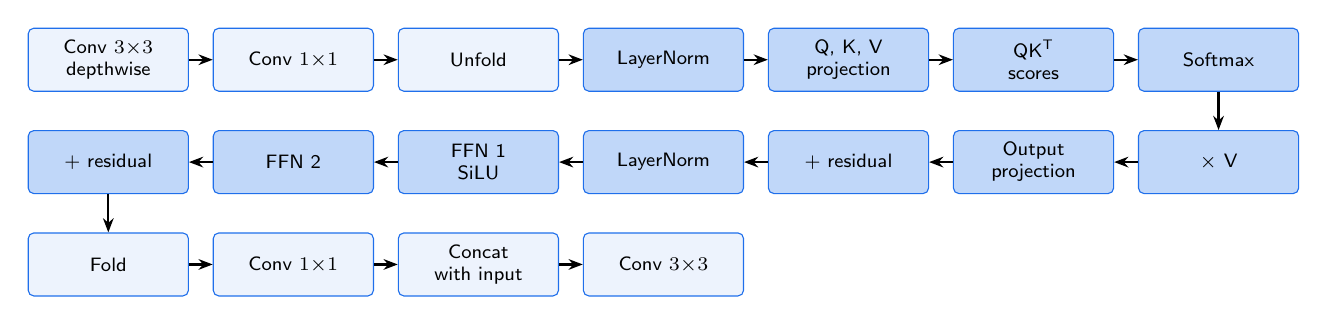
\begin{tikzpicture}[
  k/.style={draw=accent, fill=accent!8, rounded corners=2pt, minimum height=8mm,
            minimum width=19mm, text width=18mm, align=center, font=\sffamily\scriptsize},
  t/.style={k, fill=accent!28},
  arr/.style={-{Stealth[length=1.8mm]}, thick}]
\foreach \n/\s/\l [count=\i from 0] in
  {a0/k/{Conv $3{\times}3$\\depthwise}, a1/k/{Conv $1{\times}1$}, a2/k/Unfold,
   a3/t/LayerNorm, a4/t/{Q, K, V\\projection}, a5/t/{QK$^\mathsf{T}$\\scores}, a6/t/Softmax}
  \node[\s] (\n) at (\i*23.5mm, 0) {\l};
\foreach \n/\s/\l [count=\i from 0] in
  {b6/t/{$\times$ V}, b5/t/{Output\\projection}, b4/t/{+ residual}, b3/t/LayerNorm,
   b2/t/{FFN 1\\SiLU}, b1/t/{FFN 2}, b0/t/{+ residual}}
  \node[\s] (\n) at ({(6-\i)*23.5mm}, -13mm) {\l};
\foreach \n/\l [count=\i from 0] in
  {c0/Fold, c1/{Conv $1{\times}1$}, c2/{Concat\\with input}, c3/{Conv $3{\times}3$}}
  \node[k] (\n) at (\i*23.5mm, -26mm) {\l};
\foreach \x/\y in {a0/a1,a1/a2,a2/a3,a3/a4,a4/a5,a5/a6,a6/b6,b6/b5,b5/b4,b4/b3,b3/b2,b2/b1,b1/b0,b0/c0,c0/c1,c1/c2,c2/c3}
  \draw[arr] (\x) -- (\y);
\end{tikzpicture}
\caption{\label{fig:mvit}A MobileViT-S transformer layer. Dark boxes: the transformer block, run twice.}
\end{figure}

Each box is one kernel run; where a box lists two kernels, either implements
that step (\doc{kernels/mobilevit}{MobileViT-S kernels} lists every layer):

\begin{center}
\footnotesize\renewcommand{\arraystretch}{1.0}
\begin{tabularx}{\linewidth}{lX}
\toprule
Box & Kernels (layer 3: $d=144$, 256 tokens) \\
\midrule
Conv $3\times3$ depthwise & \texttt{depthwise\_conv\_universal} \\
Conv $1\times1$ & \texttt{pointwise\_conv\_unified} \\
Unfold & \texttt{unfold\_32x32x144} \\
LayerNorm & \texttt{layernorm\_256x144} \\
Q, K, V projection & \texttt{proj\_qkv\_144\_p4}, \texttt{matmul\_432x144\_x128} \\
QK$^\mathsf{T}$ scores & \texttt{qk\_scores\_256x36}, \texttt{attn\_scores\_km\_256x36} \\
Softmax & \texttt{softmax\_rows\_long} (query-major), \texttt{softmax\_columns} (key-major) \\
$\times$ V & \texttt{attn\_v\_256x36}, \texttt{attn\_v\_bcast\_36} \\
Output projection & \texttt{proj\_outproj\_144\_p4}, \texttt{matmul\_144x144\_x128} \\
+ residual & \texttt{residual\_add\_256x144} \\
FFN 1, FFN 2 & \texttt{proj\_ffn1\_144\_p4}, \texttt{proj\_ffn2\_144\_p4} \\
Fold & \texttt{fold\_32x32x144} \\
Concat & \texttt{concat\_32x32x96x96} \\
Conv $3\times3$ & \texttt{conv\_universal} \\
\bottomrule
\end{tabularx}
\end{center}

%======================================================================
\section{The IPU architecture}\label{sec:arch}

Hardware specifications: \doc{specs/stage-control}{control stage},
\doc{specs/stage-accumulator}{accumulator stage}, \doc{specs/stage-aaq-str}{AAQ and store stages},
\doc{specs/cache-unit}{cache unit}, \doc{specs/riscv-host-integration}{RISC-V host integration}.

\subsection{System}

\begin{figure}[H]\centering
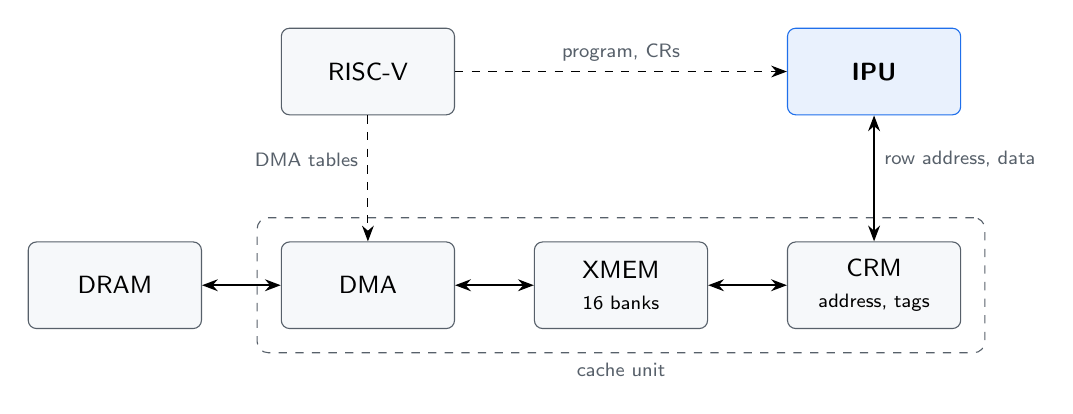
\begin{tikzpicture}[
  blk/.style={draw=accent, fill=accent!10, rounded corners=3pt, minimum height=11mm,
              minimum width=22mm, align=center, font=\sffamily\small},
  ext/.style={draw=muted, fill=outbg, rounded corners=3pt, minimum height=11mm,
              minimum width=22mm, align=center, font=\sffamily\small},
  dp/.style={{Stealth[length=2mm]}-{Stealth[length=2mm]}, thick},
  ctl/.style={-{Stealth[length=2mm]}, dashed},
  lab/.style={font=\sffamily\scriptsize, text=muted}]
\node[ext] (dram) {DRAM};
\node[ext, right=10mm of dram] (dma) {DMA};
\node[ext, right=10mm of dma] (xmem) {XMEM\\\scriptsize 16 banks};
\node[ext, right=10mm of xmem] (crm) {CRM\\\scriptsize address, tags};
\node[blk, above=16mm of crm] (ipu) {\textbf{IPU}};
\node[ext, above=16mm of dma] (riscv) {RISC-V};
\draw[dp] (dram) -- (dma);
\draw[dp] (dma) -- (xmem);
\draw[dp] (xmem) -- (crm);
\draw[dp] (ipu) -- node[lab, right, pos=0.35]{row address, data} (crm);
\draw[ctl] (riscv) -- node[lab, above]{program, CRs} (ipu);
\draw[ctl] (riscv) -- node[lab, left, pos=0.35]{DMA tables} (dma);
\begin{scope}[on background layer]
\node[draw=muted, dashed, rounded corners=4pt, inner sep=3mm, fit=(dma)(xmem)(crm),
      label={[lab]below:cache unit}] {};
\end{scope}
\end{tikzpicture}
\caption{The IPU in its system (solid: data, dashed: control).}
\end{figure}

\subsection{The pipeline}

\begin{figure}[H]\centering
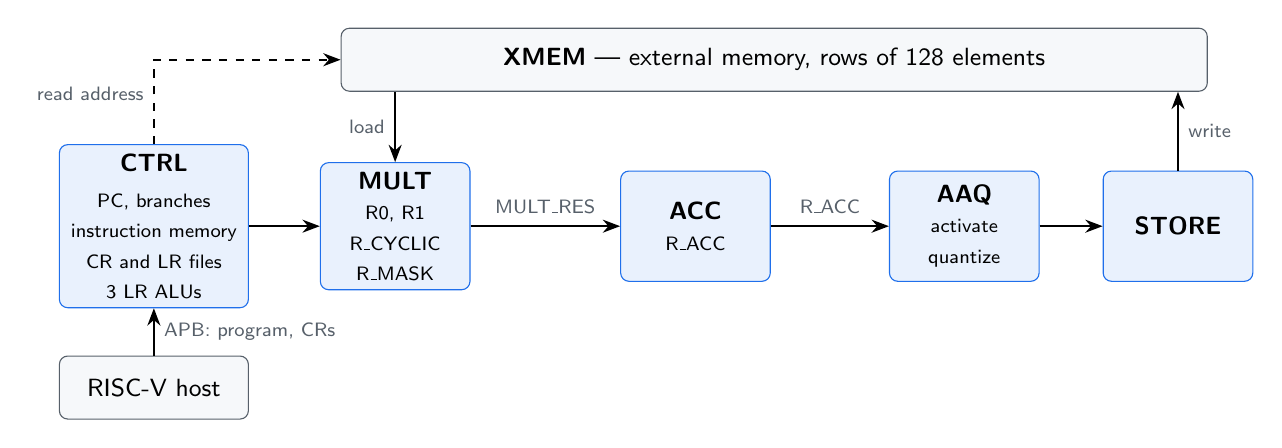
\begin{tikzpicture}[
  stage/.style={draw=accent, fill=accent!10, rounded corners=3pt, minimum height=14mm,
                minimum width=19mm, align=center, font=\sffamily\small},
  mem/.style={draw=muted, fill=outbg, rounded corners=3pt, minimum height=8mm,
              align=center, font=\sffamily\small},
  arr/.style={-{Stealth[length=2.2mm]}, thick},
  lab/.style={font=\sffamily\scriptsize, text=muted}]
\node[stage, minimum width=24mm, minimum height=20mm] (ctrl)
  {\textbf{CTRL}\\[2pt]\scriptsize PC, branches\\\scriptsize instruction memory\\\scriptsize CR and LR files\\\scriptsize 3 LR ALUs};
\node[stage, right=9mm of ctrl] (mult) {\textbf{MULT}\\\scriptsize R0, R1\\\scriptsize R\_CYCLIC\\\scriptsize R\_MASK};
\node[stage, right=19mm of mult] (acc) {\textbf{ACC}\\\scriptsize R\_ACC};
\node[stage, right=15mm of acc] (aaq) {\textbf{AAQ}\\\scriptsize activate\\\scriptsize quantize};
\node[stage, right=8mm of aaq] (st) {\textbf{STORE}};
\node[mem, above=10mm of acc, minimum width=110mm, xshift=10mm] (xmem) {\textbf{XMEM} --- external memory, rows of 128 elements};
\node[mem, below=6mm of ctrl, minimum width=24mm] (host) {RISC-V host};
\draw[arr] (host) -- node[lab, right]{APB: program, CRs} (ctrl);
\draw[arr] (ctrl) -- (mult);
\draw[arr] (mult) -- node[lab, above=1pt]{MULT\_RES} (acc);
\draw[arr] (acc) -- node[lab, above=1pt]{R\_ACC} (aaq);
\draw[arr] (aaq) -- (st);
\draw[arr, dashed] (ctrl.north) |- node[lab, pos=0.3, left]{read address} (xmem.west);
\draw[arr] (xmem.south -| mult.north) -- node[lab, left]{load} (mult.north);
\draw[arr] (st.north) -- node[lab, right]{write} (xmem.south -| st.north);
\end{tikzpicture}
\caption{The pipeline. CTRL issues one instruction word per cycle.}
\end{figure}

\subsection{Memory}

\textbf{XMEM} is the external memory. Assembly addresses it in \emph{rows} of
128 elements; a load reads one row, a store writes one row.

\begin{itemize}
\item \textbf{Elements.} In hardware, stored as 8-bit values plus a per-row
  scale; loads and stores convert to and from 32 bits.
\item \textbf{Addresses.} Row \texttt{CR + LR}: the host sets the base CR, the
  kernel steps the offset LR.
\item \textbf{Banks.} 16 banks of 1024 rows, filled from DRAM by DMA
  (\doc{specs/cache-unit}{cache unit}). Accessing a bank before DMA has filled
  all of it stalls the IPU.
\end{itemize}

\needspace{7cm}
\subsection{Registers}

Every data element is 32 bits. \texttt{CR0} = 0 and \texttt{CR1} = 1 are fixed.

\begin{center}
\begin{tabularx}{\linewidth}{l>{\raggedright\arraybackslash}p{0.28\linewidth}X}
\toprule
Register & Holds & Role \\
\midrule
\texttt{R0}, \texttt{R1} & 128 elements each & multiply-stage operands \\
\texttt{R\_CYCLIC} & 512 elements & ring of four 128-element slots \\
\texttt{R\_MASK} & 8 masks of 128 bits & one enable bit per lane \\
\texttt{MULT\_RES} & 128 $\times$ 32-bit & result of the multiply stage \\
\texttt{R\_ACC} & 128 $\times$ 32-bit & accumulator \\
\texttt{POST\_AAQ\_REG} & 128 $\times$ 32-bit & activated result \\
\texttt{LR0}--\texttt{LR15} & 16 $\times$ 32-bit & loop registers, written only by
the program \\
\texttt{CR0}--\texttt{CR15} & 16 $\times$ 32-bit & control registers, written by the
host before the run; read-only to the program \\
\bottomrule
\end{tabularx}
\end{center}

A \textbf{dstructure} CR holds \texttt{valid\_elements}, \texttt{partition}
and \texttt{pad\_mode} (section~\ref{sec:masks}); conventionally \texttt{CR15},
but each instruction names its own.

\subsection{Instruction words and slots}

The IPU is a VLIW machine: every cycle it issues one instruction \emph{word},
which holds up to one instruction per slot. In assembly, \texttt{;} separates
instructions of the same word and \texttt{;;} ends the word.

\begin{center}
\small
\begin{tabularx}{\linewidth}{l>{\raggedright\arraybackslash}p{0.3\linewidth}>{\raggedright\arraybackslash}X}
\toprule
Slot & Does & Instructions \\
\midrule
\texttt{load} & a memory row into \texttt{R0}, \texttt{R1}, \texttt{R\_CYCLIC} or \texttt{R\_MASK} & \texttt{LDR\_MULT\_REG}, \texttt{LDR\_CYCLIC\_MULT\_REG}, \texttt{LDR\_MULT\_MASK\_REG} \\
\texttt{mult} & 128-lane multiply into \texttt{MULT\_RES} & \texttt{MULT.VE}, \texttt{MULT.EE}, \texttt{MULT.RC.VV}, \texttt{MULT.RC.VE}, \texttt{MULT.RC.VS} \\
\texttt{acc} & \texttt{MULT\_RES} into \texttt{R\_ACC}: add, subtract, max; across lanes (\texttt{AGG}); decimate, scatter & \texttt{ACC.ADD}, \texttt{ACC.SUB}, \texttt{ACC.MAX} (each also \texttt{.FIRST}); \texttt{AGG.SUM}, \texttt{AGG.MAX} (also \texttt{.FIRST}); \texttt{ACC.STRIDE}, \texttt{ACC.RESHAPE} \\
\texttt{aaq} & activate and quantize \texttt{R\_ACC} into \texttt{POST\_AAQ\_REG} & \texttt{ACTIVATE.QUANTIZE} \\
\texttt{store} & writes \texttt{POST\_AAQ\_REG} to memory & \texttt{STR\_POST\_AAQ\_REG}; simulation only: \texttt{STR\_ACC\_REG} \\
\texttt{lr} (three) & LR arithmetic: addresses, counters & \texttt{SET}, \texttt{ADD}, \texttt{SUB}, \texttt{INC}, \texttt{DEC}, \texttt{INCR\_MOD\_POW2}, \texttt{ADDB}, \texttt{ADDBI} \\
\texttt{cond} & branches & \texttt{BEQ}, \texttt{BNE}, \texttt{BLT}, \texttt{BGE}, \texttt{BR}, \texttt{BKPT} \\
\texttt{break} & debugger stops & \texttt{BREAK}, \texttt{BREAK.IFEQ} \\
\bottomrule
\end{tabularx}
\end{center}

Empty slots are filled with \texttt{NOP}.
The \doc{instructions}{Instruction Reference} documents every instruction, and
\doc{assembly-syntax}{Assembly Syntax} the full syntax.

\needspace{7cm}
\subsection{Example loop}

The loop of the \texttt{identity} kernel, which copies rows:

\begin{pycode}
row_loop:
    LDR_MULT_REG r0 lr1 cr2 ;;          # load:  row CR2+LR1 -> R0
    MULT.VE lr0 cr1 0 lr0 cr15 ;        # mult:  R0 x 1.0
    ACC.ADD.FIRST ;;                    # acc:   R_ACC = MULT_RES
    ACTIVATE.QUANTIZE identity cr15 ;   # aaq:   pass through
    STR_POST_AAQ_REG lr1 cr3 ;;         # store: to row CR3+LR1
    ADD lr1 lr1 cr1 ;;                  # lr:    next row
    BLT lr1 cr4 row_loop ;;             # cond:  loop while LR1 < CR4
\end{pycode}

Each \texttt{;;} ends an instruction word, so this loop takes five cycles per
row. Faster kernels pack more work into each word --- for example loading the
next row in the same word that multiplies the current one
(section~\ref{sec:onerow}).

\subsection{Instruction memory}

Two banks of 128 words (\doc{specs/stage-control}{control stage}): the IPU
runs from one while the host loads the other. Jinja template loops (section~\ref{sec:newkernel}) unroll at assembly, so
each iteration costs words.

%======================================================================
\section{The instruction set}\label{sec:isa}

Operands are separated by spaces. The \doc{instructions}{Instruction Reference}
lists every encoding.

\subsection{Rows and elements}

XMEM operands count \textbf{rows}. Register operands count \textbf{elements}:
\texttt{R\_CYCLIC} 0--511; \texttt{R0}:\texttt{R1} 0--255, with \texttt{R1}
from 128.

\subsection{Loads}

One per word. \texttt{offset} and \texttt{index} are LRs, \texttt{base} a CR.

\begin{center}
\small
\begin{tabularx}{\linewidth}{>{\raggedright\arraybackslash}p{0.43\linewidth}>{\raggedright\arraybackslash}X}
\toprule
Syntax & Effect \\
\midrule
\texttt{LDR\_MULT\_REG R0|R1 offset base} & row $\rightarrow$ \texttt{R0} or
\texttt{R1} \\
\texttt{LDR\_CYCLIC\_MULT\_REG offset base index} & row $\rightarrow$ ring
elements \texttt{index} \ldots\ \texttt{index}+127; \texttt{index} holds 0, 128,
256 or 384 \\
\texttt{LDR\_MULT\_MASK\_REG offset base} & eight 128-bit lane masks from the
start of the row $\rightarrow$ \texttt{R\_MASK} \\
\bottomrule
\end{tabularx}
\end{center}

\subsection{Multiplies}

One per word. Each form writes 128 products to \texttt{MULT\_RES}, then masks
them (section~\ref{sec:masks}). Common operands: \texttt{m} mask number 0--7,
\texttt{sh} LR holding the mask shift, \texttt{d} dstructure CR. \texttt{rc}
and \texttt{ra} are LRs holding element numbers. RC is \texttt{R\_CYCLIC}, RA is
\texttt{R0}:\texttt{R1}.

\begin{center}
\small
\begin{tabularx}{\linewidth}{>{\raggedright\arraybackslash}p{0.36\linewidth}>{\raggedright\arraybackslash}X}
\toprule
Syntax & Lane $i$ of \texttt{MULT\_RES} \\
\midrule
\texttt{MULT.RC.VV rc R0|R1 m sh d} & $\mathrm{RC}[(rc+i) \bmod 512] \times
\mathrm{R}[i]$ \\
\texttt{MULT.RC.VE rc src m sh d} & $\mathrm{RC}[(rc+i) \bmod 512] \times s$ \\
\texttt{MULT.RC.VS rc m sh d} & $\mathrm{RC}[(rc+i) \bmod 512]^2$ \\
\texttt{MULT.VE ra cr m sh d} & $\mathrm{RA}[(ra+i) \bmod 256] \times
\mathrm{CR}$ \\
\texttt{MULT.EE ra cr m sh d} & $\mathrm{RA}[ra \bmod 256] \times \mathrm{CR}$,
every lane \\
\bottomrule
\end{tabularx}
\end{center}

\begin{itemize}
\item \textbf{Scalar $s$.} An LR \texttt{src} selects element
  $\mathrm{RA}[\mathrm{LR}]$. A CR scalar is the CR's low byte as a signed
  integer, $-128$ to $127$: \texttt{CR1} multiplies by 1.
\item \textbf{Fractions.} $0.5$ or $\log_2 e$ go in a constant row, loaded into
  \texttt{R0} or \texttt{R1} once and used with \texttt{MULT.RC.VV} or an LR
  \texttt{src}.
\end{itemize}

\begin{figure}[H]\centering
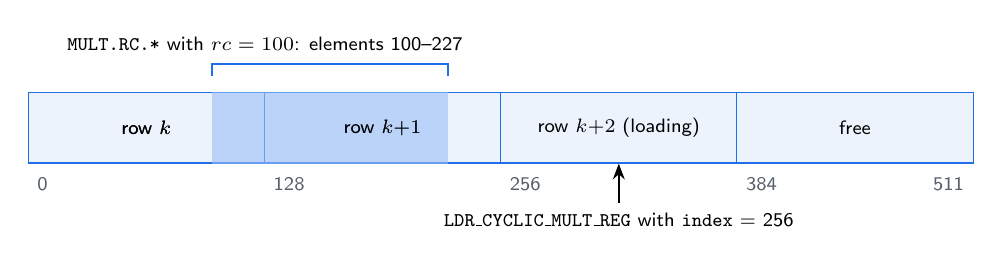
\begin{tikzpicture}[
  slot/.style={draw=accent, fill=accent!8, minimum height=9mm, minimum width=30mm,
               font=\sffamily\scriptsize, align=center},
  lab/.style={font=\sffamily\scriptsize, text=muted}]
\foreach \i/\t in {0/row $k$, 1/row $k{+}1$, 2/row $k{+}2$ (loading), 3/free}
  \node[slot] (s\i) at (\i*30mm, 0) {\t};
\foreach \i/\a in {0/0, 1/128, 2/256, 3/384}
  \node[lab, anchor=north west] at ($(s\i.south west)+(0,-0.5mm)$) {\a};
\node[lab, anchor=north east] at ($(s3.south east)+(0,-0.5mm)$) {511};
\fill[accent!45, opacity=0.6] ($(s0.north west)+(23.4mm,0)$) rectangle
  ($(s1.south west)+(23.4mm,0)$);
\foreach \i/\t in {0/row $k$, 1/row $k{+}1$}
  \node[font=\sffamily\scriptsize, align=center] at (s\i) {\t};
\draw[thick, accent] ($(s0.north west)+(23.4mm,2mm)$) -- ++(0,1.5mm) -|
  ($(s1.north west)+(23.4mm,2mm)$);
\node[lab, text=black, above] at ($(s0.north east)+(0,4mm)$)
  {\texttt{MULT.RC.*} with $rc = 100$: elements 100--227};
\draw[-{Stealth[length=2mm]}, thick] ($(s2.south)+(0,-5mm)$) -- (s2.south);
\node[lab, text=black, below] at ($(s2.south)+(0,-5mm)$)
  {\texttt{LDR\_CYCLIC\_MULT\_REG} with \texttt{index} = 256};
\end{tikzpicture}
\caption{\texttt{R\_CYCLIC}: loads fill whole slots, multiplies read any
128-element window.}
\end{figure}

\subsection{Masks and partitions}\label{sec:masks}

\begin{enumerate}
\item \texttt{m} selects one of the eight masks in \texttt{R\_MASK}.
\item The LR \texttt{sh} shifts the mask by $-3$ to $+3$ lanes. With
  \texttt{partition} $P$ (2, 4, 8 or 16), the lanes form $P$ groups of $128/P$
  and a shift stays inside each group: $+$ clears each group's first lane, $-$
  its last. $P = 0$ is one group of 128.
\item Lanes with a 0 bit take the \texttt{pad\_mode} value: 0, $+\infty$ or
  $-\infty$ ($-\infty$ ahead of a max).
\end{enumerate}

\begin{figure}[H]\centering
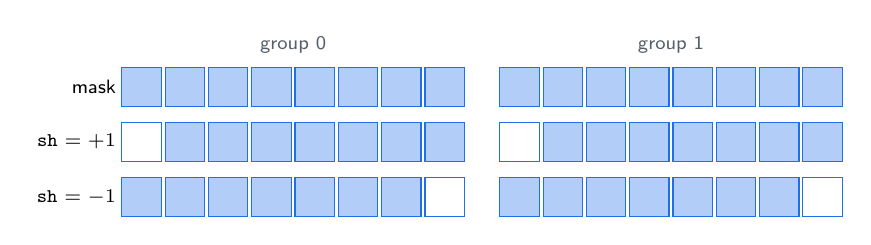
\begin{tikzpicture}[
  on/.style={draw=accent, fill=accent!35, minimum size=5mm, inner sep=0},
  off/.style={draw=accent, fill=white, minimum size=5mm, inner sep=0},
  lab/.style={font=\sffamily\scriptsize, anchor=east}]
\newcommand{\lanes}[3]{% y, label, list of 16 bits
  \node[lab] at (-2mm, #1) {#2};
  \foreach \b [count=\i from 0] in {#3} {
    \pgfmathsetmacro{\x}{\i*5.5 + (\i>7 ? 4 : 0)}
    \ifnum\b=1 \node[on] at (\x mm, #1) {}; \else \node[off] at (\x mm, #1) {}; \fi
  }}
\lanes{0}{mask}{1,1,1,1,1,1,1,1,1,1,1,1,1,1,1,1}
\lanes{-7mm}{\texttt{sh} $= +1$}{0,1,1,1,1,1,1,1,0,1,1,1,1,1,1,1}
\lanes{-14mm}{\texttt{sh} $= -1$}{1,1,1,1,1,1,1,0,1,1,1,1,1,1,1,0}
\node[font=\sffamily\scriptsize, text=muted, above] at (19.25mm, 3mm) {group 0};
\node[font=\sffamily\scriptsize, text=muted, above] at (67.25mm, 3mm) {group 1};
\end{tikzpicture}
\caption{Mask shift inside partition groups (8 lanes per group drawn). In a
$3\times3$ convolution with one image row per group, $\pm 1$ clears the edge
column.}
\end{figure}

\texttt{valid\_elements} sets the lanes \texttt{AGG} reduces and
\texttt{ACTIVATE.QUANTIZE} writes. A multiply costs one word whatever its mask.

\needspace{6cm}
\subsection{Accumulator}

One per word. One \texttt{R\_ACC}: one output row at a time.

\begin{center}
\small
\begin{tabularx}{\linewidth}{>{\raggedright\arraybackslash}p{0.36\linewidth}>{\raggedright\arraybackslash}X}
\toprule
Syntax & Effect \\
\midrule
\texttt{ACC.ADD}, \texttt{ACC.SUB}, \texttt{ACC.MAX} & per lane:
\texttt{R\_ACC} op \texttt{MULT\_RES} \\
\texttt{\ldots .FIRST} & \texttt{R\_ACC} $\leftarrow$ \texttt{MULT\_RES}
($-$\texttt{MULT\_RES} for \texttt{SUB}); starts a new result \\
\texttt{AGG.SUM LRd d}, \texttt{AGG.MAX LRd d} & sum or max of lanes 0 \ldots\
\texttt{valid\_elements}$-1$, into \texttt{R\_ACC[LRd mod 128]};
\texttt{.FIRST} overwrites, otherwise accumulates \\
\texttt{ACC.STRIDE w h v LR} & \texttt{MULT\_RES} as rows of \texttt{w} = 16, 32
or 64; \texttt{h}/\texttt{v}: \texttt{off}, \texttt{on} (even columns/rows),
\texttt{on\_inv} (odd); result into \texttt{R\_ACC} from lane
$(\mathrm{LR} \bmod 4) \times 32$ \\
\texttt{ACC.RESHAPE LRDs LRDd m} & for $j = m \ldots 7$:
\texttt{R\_ACC}$[d_j] \leftarrow$ \texttt{MULT\_RES}$[s_j]$; $s_j$, $d_j$ are
the bytes of the two pairs \\
\bottomrule
\end{tabularx}
\end{center}

\subsection{Activation and store}

\begin{center}
\small
\begin{tabularx}{\linewidth}{>{\raggedright\arraybackslash}p{0.43\linewidth}>{\raggedright\arraybackslash}X}
\toprule
Syntax & Effect \\
\midrule
\texttt{ACTIVATE.QUANTIZE fn d} & $f(\texttt{R\_ACC}[i]) \rightarrow$
\texttt{POST\_AAQ\_REG}, lanes 0 \ldots\ \texttt{valid\_elements}$-1$ \\
\texttt{STR\_POST\_AAQ\_REG offset base} & \texttt{POST\_AAQ\_REG}
$\rightarrow$ row \texttt{base + offset} \\
\bottomrule
\end{tabularx}
\end{center}

\texttt{fn}: \texttt{identity}, \texttt{relu}, \texttt{relu6},
\texttt{sigmoid}, \texttt{tanh}, \texttt{gelu}, \texttt{softplus},
\texttt{elu}, \texttt{exp2}, \texttt{reciprocal}, \texttt{rsqrt},
\texttt{silu}, \texttt{window}.

\needspace{6\baselineskip}
\begin{itemize}
\item $e^x = \mathtt{exp2}(x \log_2 e)$: multiply by $\log_2 e$, then
  \texttt{exp2}.
\item \texttt{reciprocal}: softmax's $1/\mathrm{sum}$. \texttt{rsqrt}: layer
  norm's $1/\sigma$.
\item Stored lanes from \texttt{valid\_elements} on are undefined.
\end{itemize}

\begin{openq}
The AAQ specification has \texttt{ACTIVATE.QUANTIZE} write XMEM itself, with no
\texttt{STR\_POST\_AAQ\_REG}.
\end{openq}

\subsection{LR arithmetic}

Three per word; 32-bit, wrapping.

\begin{center}
\small
\begin{tabularx}{\linewidth}{>{\raggedright\arraybackslash}p{0.36\linewidth}>{\raggedright\arraybackslash}X}
\toprule
Syntax & Effect \\
\midrule
\texttt{SET LRd CR} & \texttt{LRd} $\leftarrow$ \texttt{CR} \\
\texttt{ADD LRd LRa LR|CR}, \texttt{SUB \ldots} & \texttt{LRd} $\leftarrow$
\texttt{LRa} $\pm$ operand \\
\texttt{INC LRd n}, \texttt{DEC LRd n} & \texttt{LRd} $\leftarrow$
\texttt{LRd} $\pm n$, $n$ = 0--255 \\
\texttt{INCR\_MOD\_POW2 LRd LR|CR k} & \texttt{LRd} $\leftarrow$
$(\texttt{LRd} + \mathrm{step}) \bmod 2^k$, $k$ = 1--9 ($k = 9$: ring pointer) \\
\texttt{ADDB LRDn LR|CR}, \texttt{ADDBI LRDn b} & signed byte added to all eight
bytes of \texttt{LRD}$n$ = \texttt{LR}$n{+}1$:\texttt{LR}$n$, clamped to 0--255 \\
\bottomrule
\end{tabularx}
\end{center}

\begin{itemize}
\item One write per LR per word; a pair counts as both registers.
\item Constants come from CRs, products included: compute them on the host.
\end{itemize}

\subsection{Branches}

One per word. \texttt{BEQ}, \texttt{BNE}, \texttt{BLT}, \texttt{BGE a b label}:
\texttt{a}, \texttt{b} are LRs or CRs, compared signed. \texttt{BR reg} jumps to
a register's value; \texttt{BKPT} ends the program. \texttt{BGT}, \texttt{BLE},
\texttt{BZ}, \texttt{BNZ} and \texttt{B} assemble into these. A taken branch
executes its target in the next cycle.

%======================================================================
\section{Timing within a word}\label{sec:timing}

The slots of a word run in this order: the three \texttt{lr}
slots, \texttt{load}, \texttt{mult}, \texttt{acc}, \texttt{aaq},
\texttt{store}, \texttt{cond}. Some reads see a result written earlier in
the same word; others see the value from the start of the cycle.

\begin{center}
\small
\begin{tabularx}{\linewidth}{lX}
\toprule
Read & Value it sees \\
\midrule
\texttt{R0}, \texttt{R1}, \texttt{R\_CYCLIC} by \texttt{mult} & start of the
cycle: a row loaded in this word reaches the multiplier one word later \\
\texttt{MULT\_RES} by \texttt{acc} & this word's multiply (except
\texttt{ACC.RESHAPE}, which reads the start-of-cycle value) \\
\texttt{R\_ACC} by \texttt{aaq} & this word's accumulate \\
\texttt{POST\_AAQ\_REG} by \texttt{store} & this word's activation \\
LR operands of \texttt{load}, \texttt{mult}, \texttt{store} & this
word's \texttt{lr} updates \\
LR and CR sources of \texttt{lr} and \texttt{cond} & start of the cycle: two
chained \texttt{ADD}s take two words \\
\bottomrule
\end{tabularx}
\end{center}

\subsection{Consequences for loops}

\begin{itemize}
\item \textbf{Branches compare the pre-update value.} With
  \texttt{ADD LR1 LR1 CR1 ; BLT LR1 CR4 loop ;;} and \texttt{LR1} starting at 0,
  the loop runs \texttt{CR4}$+1$ times; start at 1 for \texttt{CR4} times.
\item \textbf{Load and store addresses include this word's \texttt{ADD}.} To
  store row $i$ while advancing its pointer, start the pointer one lower.
\item \textbf{The epilogue fits one word}: last accumulate, activation, store.
\item \textbf{\texttt{AGG}} reads its destination LR at the start of the
  cycle.
\end{itemize}

%======================================================================
\section{Installing}

\subsection{What you need}

\begin{center}
\begin{tabularx}{\linewidth}{lX}
\toprule
Tool & Why \\
\midrule
Linux or WSL2 & the build runs on Linux; on Windows use WSL2 with Ubuntu \\
Bazelisk & installs and runs the right Bazel version; provides the \texttt{bazel} command \\
Git & to get the code \\
C/C++ compiler (\texttt{gcc}) & Bazel uses it for native build steps \\
Python 3.10 or newer & used by the build tooling; Bazel brings its own Python for the emulator \\
VS Code (optional) & with the IPU assembly extension (section~\ref{sec:vscode}): syntax colouring and error squiggles \\
\bottomrule
\end{tabularx}
\end{center}

\subsection{Windows: WSL2}

In PowerShell as administrator, then restart when asked:

\begin{termcmd}
$ wsl --install -d Ubuntu
\end{termcmd}

Open the \emph{Ubuntu} app from the Start menu, create a user, and follow the
Linux steps below inside it. Keep the repository inside the Linux file system
(e.g.\ \texttt{\textasciitilde/ipu-emulator}), not under \texttt{/mnt/c}: builds
there are much slower.

\subsection{Linux dependencies}

\begin{termcmd}
$ sudo apt-get update
$ sudo apt-get install -y build-essential git curl python3
\end{termcmd}

Bazelisk is a single file. Download it as \texttt{bazel}:

\begin{termcmd}
$ sudo curl -L -o /usr/local/bin/bazel \
    https://github.com/bazelbuild/bazelisk/releases/latest/download/bazelisk-linux-amd64
$ sudo chmod +x /usr/local/bin/bazel
\end{termcmd}

(On macOS: \texttt{brew install bazelisk}.)

\needspace{0.45\textheight}
\subsection{Verify the tools}

\needspace{11.2cm}
\begin{termcmd}
$ bazel --version
$ git --version
$ python3 --version
$ gcc --version | head -1
$ grep PRETTY_NAME /etc/os-release
\end{termcmd}

\terminal[0.5]{install_versions.png}{Tool versions (Ubuntu 24.04 under WSL2).}

\subsection{Clone and run the first test}

\begin{termcmd}
$ git clone https://github.com/rechefe/ipu-emulator.git
$ cd ipu-emulator
$ bazel test //src/tools/ipu-apps:identity
\end{termcmd}

The first build downloads Bazel's dependencies and Python packages, which
takes a few minutes; later builds reuse them.

\terminal{install_first_test.png}{The first test passing: the \texttt{identity}
kernel copies a matrix and checks the copy.}

\needspace{10\baselineskip}
\subsection{VS Code extension (optional)}\label{sec:vscode}

The IPU Assembly extension makes VS Code understand \texttt{.asm},
\texttt{.s} and \texttt{.asm.j2} files.

\begin{termcmd}
$ curl -LO https://github.com/rechefe/ipu-emulator/releases/download/vscode-latest/ipu-asm.vsix
$ code --install-extension ipu-asm.vsix
\end{termcmd}

Repeat the two commands to update. With WSL, run them in VS Code's WSL
terminal, so the extension is installed on the Linux side.

\begin{center}
\begin{tabularx}{\linewidth}{lX}
\toprule
Feature & Details \\
\midrule
Syntax colouring & instructions, registers, labels, comments, Jinja; new instructions are coloured automatically \\
Error squiggles & runs the real assembler (\texttt{ipu-as check}) on the unsaved text and underlines template, parse and encoding errors where they occur \\
Status bar & \texttt{IPU} with a check mark while checking works; \texttt{IPU: checks off} when it does not --- click it for the reason \\
\bottomrule
\end{tabularx}
\end{center}

\begin{center}
\begin{tabularx}{\linewidth}{lX}
\toprule
Name & Use \\
\midrule
\textit{IPU Assembly: Check current file} & check now \\
\textit{IPU Assembly: Why are diagnostics not running?} & explains \texttt{checks off} \\
\texttt{ipuAsm.checkCommand} & the check command; e.g.\ a virtualenv instead of Bazel: \\
 & \texttt{[".venv/bin/ipu-as", "check", "--json", "--input"]} \\
\bottomrule
\end{tabularx}
\end{center}

%======================================================================
\section{How the repository is organised}

\begin{filetree}
src/tools/
  ipu-as-py/             assembler (.asm -> .bin)
  ipu-emu-py/            emulator (runs a .bin cycle by cycle)
  ipu-common/            instruction set definition shared by both
  ipu-apps/              kernel library
    src/ipu_apps/
      kernel_registry/   finds kernels, runs cases, command-line tools
      kernels/           one folder per kernel, grouped by family
        convolutions/  matmul/  attention/  softmax/  reshape/  ...
    test/                tests that run several kernels together
docs/                    documentation site (mkdocs)
\end{filetree}

\subsection{A kernel folder}

Every kernel lives in its own folder under
\texttt{src/tools/ipu-apps/src/ipu\_apps/kernels/}. The folder name is the
kernel's name: its name in \texttt{query}, its Bazel target and its
\texttt{.asm} file name. For example \texttt{kernels/elementwise/residual\_add/}:

\begin{filetree}
residual_add/
  residual_add.asm   the IPU program
  app.py             the harness: loads XMEM, sets registers, reads output;
                     and SPEC: which computations this kernel handles
  cases.py           named inputs for the kernel, each with a NumPy check
  test.py            runs every case (and any extra tests)
  benchmark.py       optional: sizes to benchmark
\end{filetree}

The arguments of each case's \texttt{prepare} function become command-line
options of the kernel (section~\ref{sec:args}).

\subsection{Families and Bazel targets}

Folders that group kernels (\texttt{convolutions/}, \texttt{matmul/},
\ldots) are \emph{families}. Bazel targets are generated automatically from the
folders; you never edit a BUILD file to add a kernel.

\begin{center}
\begin{tabularx}{\linewidth}{lX}
\toprule
Target & What it does \\
\midrule
\texttt{:<kernel>} & \texttt{bazel run}: runs a case; \texttt{bazel test}: runs every case and \texttt{test.py} \\
\texttt{:<family>} & \texttt{bazel test}: every kernel in the family plus the family's own \texttt{test.py} \\
\texttt{:assemble\_<kernel>} & builds the kernel's \texttt{.bin} \\
\texttt{:benchmark\_<kernel>} & runs the kernel's benchmark sizes, writes \texttt{results.md} \\
\texttt{:query} & asks the registry which kernel handles a computation \\
\bottomrule
\end{tabularx}
\end{center}

%======================================================================
\section{Finding a kernel: \texttt{query}}

\subsection{List all kernels}

With no arguments, \texttt{query} lists every operation and every kernel. The
\doc{kernels}{Kernels} pages describe each family, and
\doc{app-coverage}{Application Coverage} explains how the registry picks a kernel.

\begin{termcmdtop}
$ bazel run //src/tools/ipu-apps:query
\end{termcmdtop}
\begin{termout}
Operations: attn_scores_km, attn_v, attn_v_bcast, channel_peak, concat, conv2d, depth_to_space, fold, fully_connected, identity, l2_normalize, layernorm, matmul, maxpool2d, projection, qk_scores, residual_add, sample_descriptors, score_threshold, softmax, unfold
Kernels:    89

## conv2d
- **conv1x1** -- `ipu_apps.kernels.convolutions.conv1x1.app`
...
\end{termout}

\subsection{Query an operation}

Give the operation and its parameters as \texttt{key=value}. A 3x3 depthwise
convolution over 32 channels of 64x64:

\begin{termcmdtop}
$ bazel run //src/tools/ipu-apps:query -- conv2d in_channels=32 out_channels=32 \
    kernel_size=3 stride=1 padding=1 dilation=1 groups=32 \
    has_bias=False apply_relu=False height=64 width=64
\end{termcmdtop}
\begin{termout}
SUPPORTED: kernel_size=3, groups=in_channels (depthwise), stride=1, padding=1: the universal depthwise 3x3 conv kernel (FP32). 64x64 pads internally to 64x64.
  app:  depthwise_conv_universal
  use:  ipu_apps.kernels.convolutions.depthwise_conv_universal.app.DepthwiseConvUniversalApp(inst_path=..., input_path=..., output_path=..., height=64, width=64, channels=32)
  shapes: input=(32, 64, 64), output*=(32, 64, 64), weight=(32, 1, 3, 3)   (* = derived)
\end{termout}

\begin{center}
\begin{tabularx}{\linewidth}{lX}
\toprule
Line & Meaning \\
\midrule
\texttt{SUPPORTED:} & why this kernel was chosen \\
\texttt{app:} & the kernel's name --- use it as the Bazel target \\
\texttt{use:} & the Python class and arguments, for calling it from code \\
\texttt{shapes:} & every tensor involved; \texttt{*} marks shapes the registry computed (here the output) \\
\bottomrule
\end{tabularx}
\end{center}

\needspace{9cm}
\subsection{Unsupported queries}

Every candidate kernel says why it declined. A 5x5 convolution:

\begin{termcmdtop}
$ bazel run //src/tools/ipu-apps:query -- conv2d in_channels=32 out_channels=32 \
    kernel_size=5 stride=1 padding=2 dilation=1 groups=32 \
    has_bias=False apply_relu=False height=64 width=64
\end{termcmdtop}
\begin{termout}
NOT SUPPORTED: no conv2d kernel covers this query -- conv1x1, conv3x3_relu, conv3x3_relu_cin1: needs parameter(s) 'shape', 'activation', which this query does not carry; conv_first_layer, conv_universal, conv_universal_bn_activation, conv_universal_wide384, depthwise_conv_stride2_128, depthwise_conv_stride2_16, depthwise_conv_stride2_narrow, depthwise_conv_universal, depthwise_conv_universal_bn_activation: handles only kernel_size=3; got 5; pointwise_conv_unified, pointwise_conv_unified_bn_activation: handles only kernel_size=1 (pointwise); got 5
\end{termout}

\subsection{Sweep a parameter: \texttt{--sweep}}

Replace one value by a name and sweep it over a range:

\begin{termcmdtop}
$ bazel run //src/tools/ipu-apps:query -- conv2d in_channels=8 out_channels=8 \
    kernel_size=3 stride=1 padding=1 dilation=1 groups=8 \
    has_bias=False apply_relu=False height=64 width=w --sweep w=1..200
\end{termcmdtop}
\begin{termout}
w 1..128                     depthwise_conv_universal
w 129..200                   (not covered)
\end{termout}

%======================================================================
\section{Running a kernel}

\needspace{8.6cm}
Run the kernel's default case:

\begin{termcmdtop}
$ bazel run //src/tools/ipu-apps:depthwise_conv_universal
\end{termcmdtop}
\begin{termout}
depthwise_conv_universal/default: PASS (108 cycles)
=== Run summary ===
Total cycles:             108
Mult active:               72  (66.7%)
Acc  active:               72  (66.7%)
XMEM reads:                34
XMEM writes:                9
XMEM accesses:             43
--- MAC accounting ---
Mult idle:                 36
Identity mult:              0  (0.0% of active)
Lane ops:                8464  (61.2% occupancy)
Effective MAC:          61.2%
\end{termout}

A run assembles the \texttt{.asm}; the case writes its input files; the harness
copies them into XMEM and sets the control registers; the emulator runs the
program until it halts; the harness reads the output rows back; the case checks
them against its NumPy reference. \texttt{PASS} means the output matched.

\begin{center}
\begin{tabularx}{\linewidth}{lX}
\toprule
Line & Meaning \\
\midrule
\texttt{Total cycles} & cycles until the program halted \\
\texttt{Mult / Acc active} & cycles in which the multiply / accumulate stage did work \\
\texttt{XMEM reads / writes} & external-memory row transfers \\
\texttt{Mult idle} & cycles in which the multiplier did nothing \\
\texttt{Identity mult} & multiplies by 1.0 --- data movement, not arithmetic \\
\texttt{Lane ops} & multiplier lanes that carried data, summed over cycles \\
\texttt{Effective MAC} & share of the peak multiply-accumulate rate actually used \\
\bottomrule
\end{tabularx}
\end{center}

\subsection{Cases}

\needspace{3.5cm}
\begin{termcmdtop}
$ bazel run //src/tools/ipu-apps:depthwise_conv_universal -- --list-cases
\end{termcmdtop}
\begin{termout}
default
negative_outputs
\end{termout}

\texttt{--case negative\_outputs} runs the second one.

%======================================================================
\addtocontents{toc}{\protect\newpage}
\section{Passing arguments}\label{sec:args}

\begin{note}
Arguments before \texttt{--} are for Bazel; everything after \texttt{--} goes to
the kernel.
\end{note}

\texttt{--help} lists the general options and this kernel's case options:

\begin{termcmdtop}
$ bazel run //src/tools/ipu-apps:depthwise_conv_universal -- --help
\end{termcmdtop}
\begin{termout}
options:
  --kernel KERNEL       registered kernel name
  --case CASE           named case (default: default)
  --list-cases          list cases without running
  --max-cycles MAX_CYCLES
  --profile-aliases     collect full ISA alias measurements
  --alias-report ALIAS_REPORT
                        write full ISA measurements as JSON (enables
                        profiling)
  --output OUTPUT       export completed output, including output that fails
                        validation
  --channels CHANNELS
  --height HEIGHT
  --width WIDTH
  --seed SEED
\end{termout}

\texttt{--channels}, \texttt{--height}, \texttt{--width} and \texttt{--seed}
come from this kernel's \texttt{cases.py}.

\subsection{Problem size}

\begin{termcmdtop}
$ bazel run //src/tools/ipu-apps:depthwise_conv_universal -- --channels 32 \
    --height 64 --width 64
\end{termcmdtop}
\begin{termout}
depthwise_conv_universal/default: PASS (10086 cycles)
=== Run summary ===
Total cycles:           10086
Mult active:             9216  (91.4%)
...
Effective MAC:          89.5%
\end{termout}

A larger problem keeps the pipeline busier: effective MAC rises from 61\,\%
to 89.5\,\%.

\needspace{7cm}
\subsection{Save the output}

\texttt{--output} copies the kernel's output file out of the temporary
workspace. A relative path is relative to where you ran \texttt{bazel}.

\begin{termcmdtop}
$ bazel run //src/tools/ipu-apps:depthwise_conv_universal -- \
    --channels 8 --height 32 --width 32 --output out.bin
$ ls -l out.bin
\end{termcmdtop}
\begin{termout}
depthwise_conv_universal/default: PASS (702 cycles)
...
-rw-r--r-- 1 user user 32768 Sep 23 15:31 out.bin
\end{termout}

32768 bytes = 8 channels $\times$ 32 $\times$ 32 FP32 values, in
\texttt{[channels, height, width]} order.

\subsection{Errors}

An unsupported shape is refused before anything runs:

\begin{termcmdtop}
$ bazel run //src/tools/ipu-apps:depthwise_conv_universal -- --channels 3 --width 200
\end{termcmdtop}
\begin{termout}
error: width (200) exceeds 128, the largest width this app supports
\end{termout}

\texttt{--max-cycles} stops a run that takes too long (useful for a program
that never halts):

\begin{termcmdtop}
$ bazel run //src/tools/ipu-apps:depthwise_conv_universal -- --max-cycles 50
\end{termcmdtop}
\begin{termout}
error: Exceeded 50 cycles — possible infinite loop (PC=24)
\end{termout}

%======================================================================
\section{Testing}

\texttt{bazel test} on a kernel runs every case and every test in its
\texttt{test.py}:

\needspace{6.0cm}
\begin{termcmdtop}
$ bazel test //src/tools/ipu-apps:depthwise_conv_universal
\end{termcmdtop}
\begin{termout}
    PASSED  ...test_case[depthwise_conv_universal-default] (0.7s)
    PASSED  ...test_case[depthwise_conv_universal-negative_outputs] (0.6s)
    PASSED  ...test_case[depthwise_conv_universal-channels=28,height=16,width=16] (0.6s)
    ...
    PASSED  ...test_case[depthwise_conv_universal-channels=3,height=5,width=128] (0.6s)
Test cases: finished with 11 passing, 0 skipped and 0 failing out of 11 test cases

Executed 1 out of 1 test: 1 test passes.
\end{termout}

The two named cases run first, then the extra sizes listed in the kernel's
\texttt{test.py}.

\needspace{5.6cm}
A whole family:

\begin{termcmdtop}
$ bazel test //src/tools/ipu-apps:convolutions
\end{termcmdtop}
\begin{termout}
//src/tools/ipu-apps:conv1x1                                             PASSED in 19.2s
...
//src/tools/ipu-apps:pointwise_conv_unified_bn_activation                PASSED in 33.7s

Test cases: finished with 133 passing, 0 skipped and 0 failing out of 133 test cases
Executed 15 out of 15 tests: 15 tests pass.
\end{termout}

\texttt{convolutions\_test} is the family's own \texttt{test.py}: checks that
span several kernels (routing between them, the \texttt{Conv2d} layer
adapter).

Other scopes:

\begin{termcmd}
$ bazel test //src/tools/ipu-apps:test_seam_pipeline_boundaries   # one multi-kernel test
$ bazel test //...                                                # everything
\end{termcmd}

Tests under \texttt{src/tools/ipu-apps/test/mobilevit/} run several kernels in a
row on shared memory. The \texttt{test\_full\_*} ones run a whole transformer
layer and take hours, so \texttt{bazel test //...} skips them; run them by
name, picking a variant with \texttt{--test\_arg}:

\begin{termcmd}
$ bazel test //src/tools/ipu-apps:test_full_layer_l5 --test_arg=-k \
    --test_arg=query_major
\end{termcmd}

%======================================================================
\section{Debugging}\label{sec:debug}

Add \texttt{--config=debug} to any run (reference: \doc{debugging}{Debugging}). The debugger opens stopped before the
first instruction; every argument from section~\ref{sec:args} still works.

\begin{note}
The debugger needs an interactive terminal of at least 80 columns; wider is
better.
\end{note}

\needspace{11.8cm}
Start it on \texttt{residual\_add}, which adds two tensors:

\begin{termcmd}
$ bazel run --config=debug //src/tools/ipu-apps:residual_add
\end{termcmd}

\screenshot{ra_start.png}{Just launched: paused at PC 0, cycle 0.}

The screen has four panes, numbered in their titles:

\begin{enumerate}[label=\textbf{\arabic*}]
\item \textbf{Pipeline Registers} --- R0, R1, R\_C (\texttt{R\_CYCLIC}),
  R\_MASK, R\_ACC (the accumulator) and more, one tab each.
\item \textbf{Instructions} --- the program. \texttt{\textcolor{teal}{$\blacktriangleright$}}
  marks the next instruction; lines starting \texttt{||} run in the same cycle
  as the line above (one VLIW word).
\item \textbf{XMEM} --- external memory, from row 0.
\item \textbf{CR / LR} --- control and loop registers.
\end{enumerate}

The header shows the kernel, \texttt{PAUSED}, the program counter, the cycle
count and why it stopped (\texttt{entry}, \texttt{step}, \texttt{breakpoint}).
Values that changed since the last stop are underlined.

\needspace{0.38\textheight}
\subsection{All keys}

\texttt{?} shows every key; \texttt{q} quits.

\screenshot{ra_help.png}{The help overlay (\texttt{?}; \texttt{Esc} closes it).}

\needspace{0.38\textheight}
\subsection{Stepping}

\texttt{F8} executes one instruction. After four steps:

\screenshot{ra_step.png}{\label{fig:rastep}After four \texttt{F8}: PC 4, the start of the loop.}

\needspace{0.36\textheight}
\subsection{Instruction views}

The Instructions pane has three tabs; \texttt{Tab} cycles them, \texttt{Esc}
returns to the compact one.

\screenshot[0.6]{dbg_stages.png}{The stages view at PC 0: only CTRL has work (two
\texttt{SET}s); every other stage is idle.}

\begin{center}
\begin{tabularx}{\linewidth}{lX}
\toprule
Tab & Shows \\
\midrule
\texttt{current compact} & each word's instructions, empty slots hidden \\
\texttt{current full} & every slot of each word, including \texttt{NOP}s \\
\texttt{current stages} & the word about to run, split by pipeline stage (CTRL, MULT, ACC, AAQ, STORE, XMEM input); stages with nothing to do show \texttt{IDLE} \\
\bottomrule
\end{tabularx}
\end{center}

\needspace{0.38\textheight}
\subsection{Breakpoints}

Press \texttt{2} to focus the Instructions pane, move the cursor with the arrow
keys, and press \texttt{F9} to toggle a breakpoint (a red \texttt{B}):

\screenshot{ra_bp.png}{Breakpoint set at PC 8 (\texttt{BLT}, the loop's branch).}

\needspace{0.38\textheight}
\texttt{F5} continues until a breakpoint:

\screenshot{ra_continue.png}{Stopped at the breakpoint: the header reason is
\texttt{breakpoint}.}

\texttt{F10} runs to the cursor instead. A breakpoint can also be written into
the program: \texttt{BREAK;;} always stops, \texttt{BREAK.IFEQ LR0 5;;}
stops only when \texttt{LR0} is 5.

\needspace{0.38\textheight}
\subsection{Registers and memory}

In a pane, \texttt{Tab} selects the next tab and \texttt{f} cycles the number
format. Press \texttt{F8} once more (\texttt{BLT} branches back to PC 4), then
focus the pipeline pane (\texttt{1}) and press \texttt{Tab} four times to reach
R\_ACC:

\screenshot{ra_racc_step.png}{R\_ACC as FP32 values after one loop iteration:
the sum of the first channel of A and B.}

\needspace{0.38\textheight}
Focus XMEM (\texttt{3}) and select its f32 tab to read memory as numbers:

\screenshot{ra_xmem_f32.png}{XMEM row 0 as FP32: the first channel of input A.}

\needspace{0.38\textheight}
\subsection{Edit values}

Select a value and press \texttt{e} (or double-click it). Registers take
decimal, \texttt{0x} hex or \texttt{0b} binary; XMEM and pipeline values are
entered in the tab's format. \texttt{CR0} and \texttt{CR1} are read-only.

\screenshot{dbg_edit_editor.png}{\texttt{4}, three \texttt{Down}, \texttt{e},
then \texttt{7}: setting \texttt{LR3}.}

After \texttt{Enter} the header confirms \texttt{Set LR3 = 0x7}, and XMEM tabs
that use \texttt{LR3} refresh immediately.

\needspace{0.38\textheight}
\subsection{Memory tabs}

\texttt{F2} adds a tab to the focused pane. In the XMEM pane it asks for
\texttt{row|byte BASE OFFSET COUNT FORMAT}, where \texttt{BASE} and
\texttt{OFFSET} may be registers and \texttt{COUNT} is in bytes. The editor
starts with the current tab's request. Clear it and type
\texttt{row cr4 0 512 f32} --- one row (512 bytes) from the row in \texttt{CR4},
the output of \texttt{residual\_add} --- then press \texttt{Enter}:

\screenshot{dbg_f2_added.png}{A new tab shows the output
row as FP32, at byte address \texttt{0x00100000} (row 2048). The tab keeps its
symbolic request, so it follows \texttt{CR4} and \texttt{LR} values as they
change.}

The other panes take different requests:

\begin{center}
\begin{tabularx}{\linewidth}{lX}
\toprule
Pane & \texttt{F2} / \texttt{F3} value \\
\midrule
Instructions & \texttt{current}, or a fixed PC \\
CR / LR & \texttt{all}, \texttt{lr} or \texttt{cr} \\
XMEM & \texttt{row|byte BASE OFFSET COUNT FORMAT}, e.g.\ \texttt{row cr4 lr0 16 f32} \\
Pipeline Registers & a register: \texttt{R0}, \texttt{R\_ACC}, \texttt{MULT\_RES}, \texttt{MEM\_BYPASS}, \ldots \\
\bottomrule
\end{tabularx}
\end{center}

\texttt{F3} edits the current tab's request, \texttt{F4} closes the tab.
Formats: \texttt{hex}, \texttt{int8}, \texttt{u8}, \texttt{cell16},
\texttt{u32}, \texttt{int32}, \texttt{f32}, \texttt{bits} (\texttt{f} cycles
them).

\subsection{Mouse and layout}

\begin{itemize}
\item Click a value to select it; double-click to edit it.
\item Click the two left columns of an instruction to toggle a breakpoint.
\item The wheel scrolls the pane under the pointer; \texttt{Shift}-wheel scrolls sideways.
\item Drag a pane border to resize it; \texttt{Shift}+arrows do the same from
  the keyboard, \texttt{=} resets the layout.
\item Tabs, their close buttons and every footer shortcut are clickable.
\end{itemize}

%======================================================================
\section{Assembling a kernel}\label{sec:asm}

\needspace{5.6cm}
To get the binary without running it:

\begin{termcmdtop}
$ bazel build //src/tools/ipu-apps:assemble_depthwise_conv_universal
\end{termcmdtop}
\begin{termout}
Assembling file: src/tools/ipu-apps/src/ipu_apps/kernels/convolutions/depthwise_conv_universal/depthwise_conv_universal.asm
Output will be saved to: bazel-out/k8-fastbuild/bin/src/tools/ipu-apps/assemble_depthwise_conv_universal.bin
Target //src/tools/ipu-apps:assemble_depthwise_conv_universal up-to-date:
  bazel-bin/src/tools/ipu-apps/assemble_depthwise_conv_universal.bin
\end{termout}

\subsection{Standalone assembler}

\texttt{ipu-as} assembles or checks any \texttt{.asm} file. \texttt{bazel run}
runs it inside Bazel's own directory, so give \textbf{absolute} paths
(\texttt{\$PWD/...}); and pass \texttt{--format bin}, or it asks:

\begin{termcmd}
$ bazel run //src/tools/ipu-as-py:ipu-as -- assemble --format bin \
    --input $PWD/prog.asm --output $PWD/prog.bin
$ ls -l prog.bin
$ bazel run //src/tools/ipu-as-py:ipu-as -- check --input $PWD/prog.asm
$ bazel run //src/tools/ipu-as-py:ipu-as -- check --input $PWD/bad.asm
\end{termcmd}

\texttt{bad.asm} contains \texttt{BEQ lr0, cr0, +1}:

\terminal{assembler.png}{\label{fig:assembler}Operands are separated by spaces, so the comma is an error.}

\begin{center}
\begin{tabularx}{\linewidth}{lX}
\toprule
Command & Does \\
\midrule
\texttt{assemble} & \texttt{.asm} $\rightarrow$ binary (\texttt{--format bin}) or memory image (\texttt{mem}) \\
\texttt{check} & reports every error with line and column; exit code 1 on errors; \texttt{--json} for tools \\
\texttt{disassemble} & binary $\rightarrow$ assembly text \\
\bottomrule
\end{tabularx}
\end{center}

%======================================================================
\section{Writing a kernel}\label{sec:newkernel}

A complete example kernel, \texttt{double\_rows}: $y = 2x$ for a matrix of
128-element FP32 rows, built from the smallest existing kernel,
\texttt{kernels/reshape/identity/}, which copies rows.

\subsection{Create the folder}

\begin{termcmd}
$ cd src/tools/ipu-apps/src/ipu_apps/kernels
$ mkdir -p examples/double_rows
$ touch examples/__init__.py examples/double_rows/__init__.py
\end{termcmd}

\texttt{examples/} is a new family. The empty \texttt{\_\_init\_\_.py} files
mark the folders as Python packages. The folder name, \texttt{double\_rows},
becomes the kernel's name and its Bazel target.

\subsection{Program: \texttt{double\_rows.asm}}

\begin{pycode}
{# y = 2x. CR2 = input row, CR3 = output row, CR4 = row count #}
{%- set lr_zero = "lr0" -%}
{%- set lr_row  = "lr1" -%}

    SET {{lr_zero}} cr0 ;
    SET {{lr_row}} cr0 ;;

row_loop:
    LDR_MULT_REG r0 {{lr_row}} cr2 ;;
    MULT.VE {{lr_zero}} cr1 0 {{lr_zero}} cr15 ;
    ACC.ADD.FIRST ;;
    MULT.VE {{lr_zero}} cr1 0 {{lr_zero}} cr15 ;
    ACC.ADD ;;
    ACTIVATE.QUANTIZE identity cr15 ;
    STR_POST_AAQ_REG {{lr_row}} cr3 ;;
    ADD {{lr_row}} {{lr_row}} cr1 ;;
    BLT {{lr_row}} cr4 row_loop ;;
    BKPT ;;
\end{pycode}

\begin{itemize}
\item \texttt{\{\% set lr\_row = "lr1" \%\}} --- Jinja names for registers.
\item \texttt{SET lr0 cr0 ; SET lr1 cr0 ;;} --- one word, two \texttt{lr}
  slots: both start at 0.
\item \texttt{LDR\_MULT\_REG r0 lr1 cr2 ;;} --- load row \texttt{CR2 + LR1}
  (the current input row) into \texttt{R0}.
\item \texttt{MULT.VE ... cr1 ... ; ACC.ADD.FIRST ;;} --- multiply \texttt{R0}
  by \texttt{CR1} (= 1.0) and start the accumulator with it.
\item \texttt{MULT.VE ... ; ACC.ADD ;;} --- the same again, added on top:
  \texttt{R\_ACC} = $x + x = 2x$.
\item \texttt{ACTIVATE.QUANTIZE identity cr15 ; STR\_POST\_AAQ\_REG lr1 cr3 ;;}
  --- pass \texttt{R\_ACC} through unchanged and store it at output row
  \texttt{CR3 + LR1}.
\item \texttt{ADD ... ;; BLT lr1 cr4 row\_loop ;;} --- next row, loop while
  \texttt{LR1 < CR4}; \texttt{BKPT ;;} halts.
\end{itemize}

\subsection{Harness and SPEC: \texttt{app.py}}

\begin{pycode}
from ipu_emu.ipu import LANES

from ipu_apps.kernel_registry.memory import MemoryApp, MemoryLayout, memory_spec

class DoubleRowsApp(MemoryApp):
    @classmethod
    def memory_layout(cls, *, shape):
        rows, columns = tuple(shape)
        if rows < 1:
            raise ValueError(f"needs at least one row; got {rows}")
        if columns != LANES:
            raise ValueError(f"expects {LANES} columns; got {columns}")
        return MemoryLayout(rows, rows, {2: 0, 3: rows, 4: rows})

SPEC = memory_spec(
    "double", DoubleRowsApp,
    explain=lambda **params: "each element is multiplied by 2",
    caveats=lambda **params: (),
)
\end{pycode}

\texttt{MemoryApp} does the loading and unloading: the input file is copied to
XMEM from row 0, the output is read from the rows after it. Your code only
states the layout: \texttt{MemoryLayout(input\_rows, output\_rows, crs)}, with
the control registers the program reads (\texttt{CR2} input row,
\texttt{CR3} output row, \texttt{CR4} row count). A \texttt{ValueError} there
becomes a refusal in \texttt{query}. \texttt{memory\_spec("double", ...)}
registers the kernel under the operation \texttt{double}.

\subsection{Cases: \texttt{cases.py}}

\begin{pycode}
import numpy as np

from ipu_emu.ipu import LANES
from ipu_apps.kernel_registry.cases import KernelCase, PreparedCase

def prepare(workspace, *, rows, seed):
    x = np.random.RandomState(seed).uniform(-10, 10, (rows, LANES)).astype("<f4")
    inp, out = workspace / "input.bin", workspace / "output.bin"
    inp.write_bytes(x.tobytes())

    def check():
        y = np.fromfile(out, dtype="<f4").reshape(rows, LANES)
        np.testing.assert_array_equal(y, 2 * x)

    return PreparedCase({"shape": (rows, LANES)},
                        {"input_path": inp, "output_path": out}, check)

CASES = {
    "default": KernelCase(prepare, {"rows": 4, "seed": 0}),
}
\end{pycode}

\texttt{prepare} receives the case options (\texttt{rows}, \texttt{seed}), which
become the kernel's command-line options. It writes the input file and returns
the query parameters, the file paths, and \texttt{check}, which raises if the
output is wrong.

\subsection{Test: \texttt{test.py}}

\begin{pycode}
"""double_rows: every case, plus two more sizes."""
from ipu_apps.kernel_registry.testing import case_tests

test_case = case_tests(__package__, sweep=[dict(rows=1, seed=1), dict(rows=64, seed=2)])
\end{pycode}

\texttt{case\_tests} runs every case, plus the default case again with each
\texttt{sweep} override.

\needspace{0.42\textheight}
\subsection{Run it}

No BUILD file changes: the targets exist as soon as the \texttt{.asm} does.

\begin{termcmd}
$ bazel run //src/tools/ipu-apps:query -- double shape=4,128
$ bazel run //src/tools/ipu-apps:double_rows
\end{termcmd}

\terminal{ex_run.png}{The registry finds the new kernel, and the default case passes.}

\texttt{Identity mult: 100\%} and the aliases \texttt{A1\_MOV\_RC} /
\texttt{A2\_ADD\_VV}: doubling by adding a row to itself spends the multiplier
on data movement; section~\ref{sec:onerow} cuts this kernel from 386 to 67
cycles on 64 rows.

\needspace{0.3\textheight}
\subsection{Test it}

\begin{termcmd}
$ bazel test //src/tools/ipu-apps:double_rows
\end{termcmd}

\terminal{ex_test.png}{The default case and the two sweep sizes pass.}

\needspace{0.45\textheight}
\subsection{Debug it}

\begin{termcmd}
$ bazel run --config=debug //src/tools/ipu-apps:double_rows
\end{termcmd}

\screenshot{ex_steps.png}{After three \texttt{F8}: \texttt{R0} holds the first
input row (pane 1); PC 3 is about to add it a second time.}

\subsection{Checklist}

\begin{itemize}
\item Folder, \texttt{.asm} file and target share one name.
\item \texttt{app.py} defines the harness and \texttt{SPEC}; \texttt{cases.py}
  defines \texttt{CASES} with a \texttt{"default"}; \texttt{test.py} calls
  \texttt{case\_tests}.
\item \texttt{bazel test //src/tools/ipu-apps:test\_kernel\_registry} checks
  that the new kernel is registered correctly.
\item \doc{adding-applications}{Adding Applications} covers kernels whose
  harness prepares its own memory layout, and \texttt{benchmark.py}.
\end{itemize}

%======================================================================
\section{ISA aliases}\label{sec:aliases}

The IPU instruction set has gaps: there is, for example, no instruction that
adds two vectors. Kernels fill a gap with a sequence of other instructions ---
to add two vectors, multiply each by 1.0 and accumulate. Such a sequence is an
\textbf{alias}, and it costs multiplier cycles: every accumulator instruction
reads \texttt{MULT\_RES}, so any data reaching \texttt{R\_ACC} passes through
the multiplier. The \doc{isa-alias-catalogue}{ISA Alias Catalogue} lists them
as A1--A16.

\subsection{Alias counts}

\begin{termcmdtop}
$ bazel run //src/tools/ipu-apps:residual_add
\end{termcmdtop}
\begin{termout}
residual_add/default: PASS (325 cycles)
...
Identity mult:            128  (100.0% of active)
Effective MAC:           0.0%
--- ISA alias hits ---
A1_MOV_RC:                 64
A2_ADD_VV:                 64
A16_STR_ACC_REG:           64
\end{termout}

Every multiply is a multiply by 1.0 (\texttt{Identity mult: 100\%}), so no
real arithmetic happens in the multiplier (\texttt{Effective MAC: 0.0\%}).
Per channel (64 channels): one \texttt{A1\_MOV\_RC} (move A into the
accumulator), one \texttt{A2\_ADD\_VV} (add B) and one
\texttt{A16\_STR\_ACC\_REG} (store with a simulation-only instruction).

\subsection{Aliases in the debugger}

In figure~\ref{fig:rastep}, PC 4 and PC 6 are the aliases:
\texttt{MULT.RC.VE ... cr1} multiplies by \texttt{CR1} = 1.0;
\texttt{ACC.ADD.FIRST} starts the sum (A1), \texttt{ACC.ADD} adds the second
vector (A2).

\needspace{6cm}
\subsection{Alias report}

\begin{termcmdtop}
$ bazel run //src/tools/ipu-apps:residual_add -- --profile-aliases
\end{termcmdtop}
\begin{termout}
--- Full ISA measurements (overlapping; no savings estimates) ---
A2_ADD_VV/default: 64 occurrences (verified), 64 participating cycles
A1_MOV_RC/default: 64 occurrences (verified), 64 participating cycles
A16_STR_ACC_REG/default: 64 occurrences (verified), 64 participating cycles
A12_ADDRESSING/load_to_mult: 128 occurrences (verified), 256 participating cycles
A12_ADDRESSING/address_update: 64 occurrences (verified), 128 participating cycles
A13_NARROW_MULT/lanes_128: 128 occurrences (verified), 128 participating cycles
\end{termout}

\texttt{--alias-report FILE} writes the same as JSON, including where each
alias occurs (\texttt{sites}: program counter $\rightarrow$ count) and
examples:

\begin{termcmdtop}
$ bazel run //src/tools/ipu-apps:residual_add -- --alias-report aliases.json
\end{termcmdtop}
\begin{termout}
"A2_ADD_VV": {
  "name": "ADD.VV",
  "measurements": [{ "status": "verified", "count": 64, "sites": { "6": 64 },
      "examples": [{ "events": [
          { "cycle": 7, "pc": 6, "slot": "mult", "instruction": "MULT.RC.VE" },
          { "cycle": 7, "pc": 6, "slot": "acc",  "instruction": "ACC.ADD" } ] }, ...
\end{termout}

\subsection{Benchmarks}

A kernel with a \texttt{benchmark.py} runs its benchmark sizes and prints the
statistics and alias counts per size:

\begin{termcmdtop}
$ bazel run //src/tools/ipu-apps:benchmark_depthwise_conv_universal
\end{termcmdtop}
\begin{termout}
=== depthwise_conv_universal benchmark ===
config                            cycles  cyc/channels  mult%   acc%  lanes%  ident%  effMAC%
---------------------------------------------------------------------------------------------
height=16,width=16,channels=8        180         22.50  80.0%  80.0%   73.5%    0.0%    73.5%
height=64,width=64,channels=64     19686        307.59  93.6%  93.6%   91.7%    0.0%    91.7%
...
ISA aliases: A7 REDUCE_SEG  A12 ADDRESSING  A13 NARROW_MULT  A14 MULTIPLE_ACC
config                                  A7   A12    A13   A14
-------------------------------------------------------------
height=16,width=16,channels=8        0+93?    50    144    32
height=64,width=64,channels=64    0+10238?  6396  18432  4504
...
wrote .../kernels/convolutions/depthwise_conv_universal/results.md
\end{termout}

\texttt{0+93?} means 0 verified and 93 unverified candidate occurrences.

%======================================================================
\section{Making kernels faster}\label{sec:fast}

\subsection{Cost model}

One word per cycle: run time is words executed, plus bank stalls. Two ways to
cut it:

\begin{itemize}
\item \textbf{Less work}: fewer instructions per result, and multiplies that do
  arithmetic rather than $\times 1$ moves.
\item \textbf{Overlap}: independent instructions share a word and cost one
  cycle together.
\end{itemize}

The multiplier sets the peak: one 128-lane multiply per cycle.
\texttt{Effective MAC} in the run summary is the share of that peak doing real
arithmetic, excluding $\times 1$ moves and idle lanes. Target: one word per
inner-loop iteration, holding the next load, the multiply, the accumulate, the
pointer updates and the branch.

\begin{center}
\small
\begin{tabularx}{\linewidth}{lrrX}
\toprule
Kernel (default case) & Cycles & Eff.\ MAC & Inner loop \\
\midrule
\texttt{matmul\_144x144\_x128} & 43921 & 94.4\,\% & one word per step \\
\texttt{matmul\_128x128} & 34055 & 48.1\,\% & two words per step, one only
updating pointers \\
\texttt{residual\_add} & 325 & 0.0\,\% & $\times 1$ moves only \\
\texttt{softmax\_rows} & 2323 & 16.5\,\% & 40\,\% $\times 1$ moves;
load, multiply, update and branch in separate words \\
\bottomrule
\end{tabularx}
\end{center}

\subsection{Example: \texttt{double\_rows}}\label{sec:onerow}

The kernel of section~\ref{sec:newkernel}, on 64 rows:

\begin{center}
\small
\begin{tabular}{lrrrr}
\toprule
Version & Words per row & Multiplies per row & Cycles & Eff.\ MAC \\
\midrule
$x \cdot 1 + x \cdot 1$ (section~\ref{sec:newkernel}) & 6 & 2 & 386 & 0.0\,\% \\
$x \cdot 2$ & 5 & 1 & 322 & 19.9\,\% \\
$x \cdot 2$, one word per row & 1 & 1 & 67 & 95.5\,\% \\
\bottomrule
\end{tabular}
\end{center}

\textbf{Less work: multiply by 2.} The two $\times 1$ multiplies (aliases A1
and A2) become one multiply by a CR holding 2; a CR scalar is a signed integer,
so 2 is exact (section~\ref{sec:isa}). In \texttt{app.py}, set \texttt{CR5}:

\begin{pycode}
        return MemoryLayout(rows, rows, {2: 0, 3: rows, 4: rows, 5: 2})
\end{pycode}

and in \texttt{double\_rows.asm} replace the two multiply words with one:

\begin{pycode}
    MULT.VE {{lr_zero}} cr5 0 {{lr_zero}} cr15 ;
    ACC.ADD.FIRST ;;
\end{pycode}

\needspace{0.42\textheight}
\textbf{Overlap: one word per row.} Load, multiply, store, pointer update and
branch still take five words. Loading row $i+1$ while multiplying and storing
row $i$ puts them in one:

\begin{pycode}
    SET LR0 CR0 ;                       # LR0 = 0 (index and shift)
    SET LR1 CR0 ;                       # LR1 = 0
    SET LR2 CR1 ;;                      # LR2 = 1
    SUB LR3 LR1 CR1 ;                   # LR3 = -1
    LDR_MULT_REG R0 LR1 CR2 ;;          # prime: row 0 -> R0
row_loop:                               # one word per row i:
    ADD LR1 LR1 CR1 ;                   #   LR1: i -> i+1
    ADD LR2 LR2 CR1 ;                   #   LR2: i+1 -> i+2
    ADD LR3 LR3 CR1 ;                   #   LR3: i-1 -> i
    LDR_MULT_REG R0 LR1 CR2 ;           #   row i+1 -> R0, for the next word
    MULT.VE LR0 CR5 0 LR0 CR15 ;        #   row i (loaded last word) x 2
    ACC.ADD.FIRST ;
    ACTIVATE.QUANTIZE identity CR15 ;
    STR_POST_AAQ_REG LR3 CR3 ;          #   store row i
    BLT LR2 CR4 row_loop ;;             #   continue while i+1 < CR4
    BKPT ;;
\end{pycode}

\begin{itemize}
\item Load and store see this word's \texttt{ADD}s: \texttt{LR1} $= i+1$,
  \texttt{LR3} $= i$.
\item \texttt{BLT} sees \texttt{LR2} before its \texttt{ADD}: $i+1$.
\item Three counters fill the three LR slots.
\end{itemize}

\begin{figure}[H]\centering
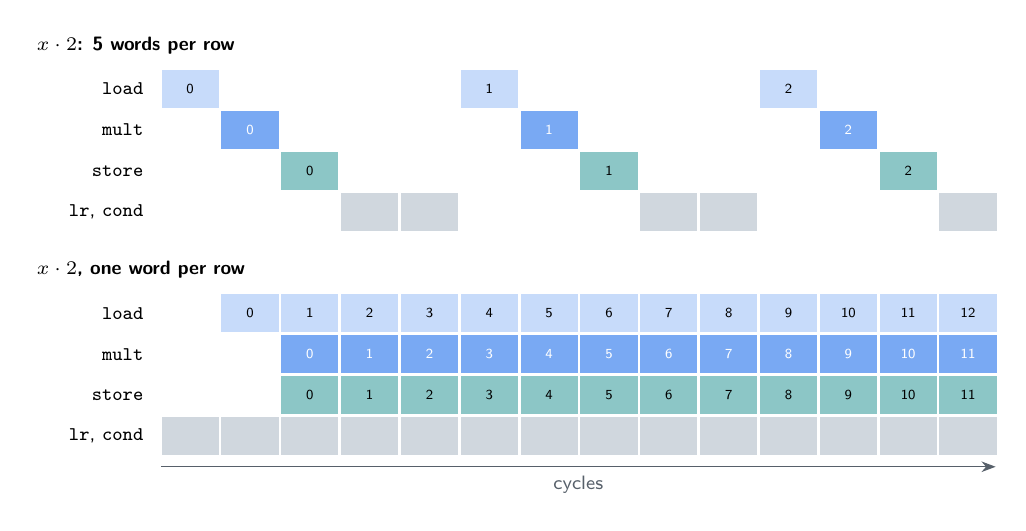
\begin{tikzpicture}[
  c/.style={draw=white, minimum width=7.4mm, minimum height=5mm, inner sep=0,
            font=\sffamily\tiny},
  L/.style={c, fill=accent!25}, M/.style={c, fill=accent!60, text=white},
  S/.style={c, fill=teal!45}, X/.style={c, fill=outframe},
  lab/.style={font=\sffamily\scriptsize, anchor=east}]
\newcommand{\track}[3]{% y, label, cells: style/text
  \node[lab] at (-1mm, #1) {#2};
  \foreach \s/\t [count=\i from 0] in {#3}
    \node[\s] at (\i*7.6mm+3.7mm, #1) {\t};}
\node[font=\sffamily\scriptsize\bfseries, anchor=west] at (-17mm, 5.5mm)
  {$x \cdot 2$: 5 words per row};
\track{0}{\texttt{load}}{L/0,c/,c/,c/,c/,L/1,c/,c/,c/,c/,L/2,c/,c/,c/}
\track{-5.2mm}{\texttt{mult}}{c/,M/0,c/,c/,c/,c/,M/1,c/,c/,c/,c/,M/2,c/,c/}
\track{-10.4mm}{\texttt{store}}{c/,c/,S/0,c/,c/,c/,c/,S/1,c/,c/,c/,c/,S/2,c/}
\track{-15.6mm}{\texttt{lr}, \texttt{cond}}{c/,c/,c/,X/,X/,c/,c/,c/,X/,X/,c/,c/,c/,X/}
\node[font=\sffamily\scriptsize\bfseries, anchor=west] at (-17mm, -23mm)
  {$x \cdot 2$, one word per row};
\track{-28.5mm}{\texttt{load}}{c/,L/0,L/1,L/2,L/3,L/4,L/5,L/6,L/7,L/8,L/9,L/10,L/11,L/12}
\track{-33.7mm}{\texttt{mult}}{c/,c/,M/0,M/1,M/2,M/3,M/4,M/5,M/6,M/7,M/8,M/9,M/10,M/11}
\track{-38.9mm}{\texttt{store}}{c/,c/,S/0,S/1,S/2,S/3,S/4,S/5,S/6,S/7,S/8,S/9,S/10,S/11}
\track{-44.1mm}{\texttt{lr}, \texttt{cond}}{X/,X/,X/,X/,X/,X/,X/,X/,X/,X/,X/,X/,X/,X/}
\draw[-{Stealth[length=1.8mm]}, muted] (0, -48mm) -- node[below,
  font=\sffamily\scriptsize, text=muted] {cycles} (106mm, -48mm);
\end{tikzpicture}
\caption{The first 14 cycles; numbers are rows.}
\end{figure}

\subsection{Techniques from the kernel library}

\textbf{Counters stay in the loop word.} \texttt{matmul\_144x144\_x128}:

\begin{pycode}
k_loop:
    MULT.RC.VE LR0 LR5 0 LR0 CR15 ;     # ring x weight R0[LR5]
    ACC.ADD ;
    LDR_CYCLIC_MULT_REG LR4 CR0 LR0 ;   # next activation row -> ring slot 0
    ADD LR4 LR4 LR2 ;                   # next row
    ADD LR5 LR5 CR1 ;                   # next weight
    BLT LR5 LR6 k_loop ;;
\end{pycode}

The multiply reads \texttt{LR5} after the \texttt{ADD}, the branch before it;
\texttt{LR5} starts one lower to suit both.

\begin{figure}[H]\centering
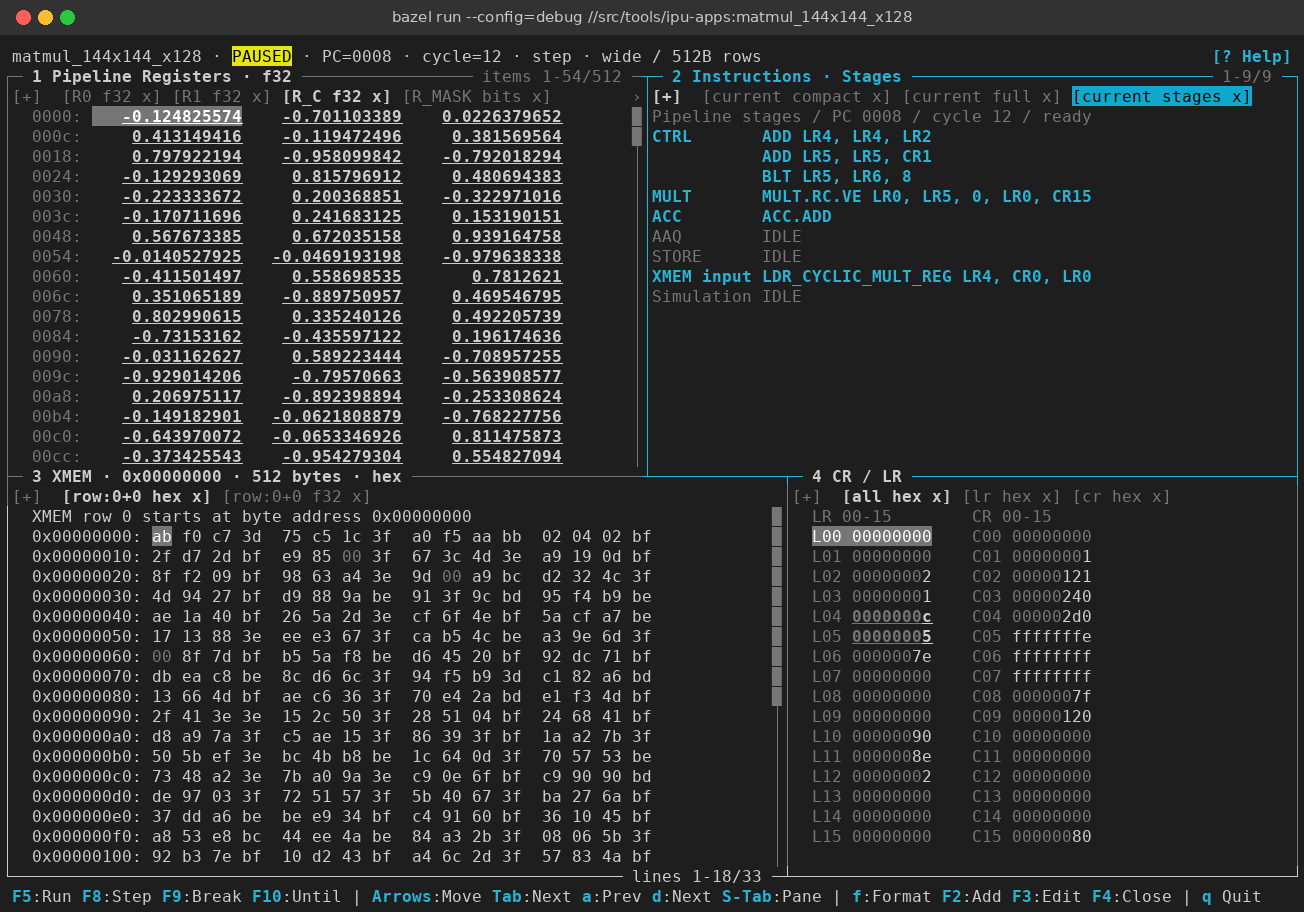
\includegraphics[width=0.72\linewidth]{images/dbg_matmul_loop.png}
\caption{The loop word in the debugger's stages view
(section~\ref{sec:debug}): CTRL, MULT, ACC and the XMEM load all work in the
same cycle.}
\end{figure}

\needspace{3\baselineskip}
\textbf{The ring as a rotating buffer.} \texttt{depthwise\_conv\_universal}
holds a $3\times3$ window's three input rows in ring slots and loads the next
channel's rows into the free slots during the current channel's taps;
\texttt{INCR\_MOD\_POW2 LR5 CR9 9} rotates the slot pointer.

\textbf{One pointer for all taps.} One \texttt{rc} register walks the nine taps:
$+1$ within a tap row, a CR step between rows. A mask shift of $\pm 1$ clears the
left and right image edges, with \texttt{partition} grouping lanes into image
rows; dedicated masks in \texttt{R\_MASK} clear the top and bottom rows.

\textbf{Epilogue in the last tap.} The last accumulate and
\texttt{ACTIVATE.QUANTIZE} share the ninth tap's word. That word's three LR
slots are full, so the store and its pointer \texttt{ADD} go into the next
channel's second tap: 9 words per channel, down from 11.

\textbf{Packed lanes.} The convolutions pack $128/W$ image rows of width
$W \in \{16, 32, 64, 128\}$ into one XMEM row. The depthwise kernel packs the
nine weights of 28 channels ($28 \times 9 = 252$) into
\texttt{R0}:\texttt{R1}.

%======================================================================
\section{Data layout in XMEM}\label{sec:layout}

A multiply consumes one 128-element row, so the layout decides which dimension
runs across the lanes.

\begin{figure}[H]\centering
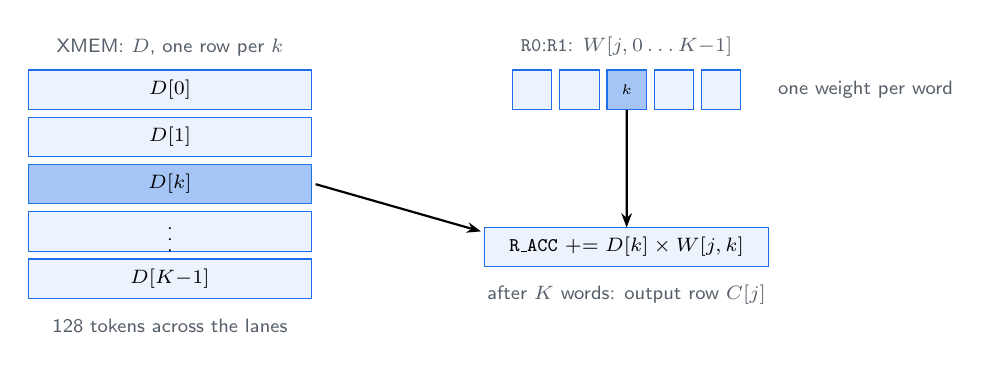
\begin{tikzpicture}[
  row/.style={draw=accent, fill=accent!8, minimum height=5mm, minimum width=36mm,
              inner sep=0, font=\sffamily\scriptsize},
  hot/.style={row, fill=accent!40},
  cell/.style={draw=accent, fill=accent!8, minimum size=5mm, inner sep=0,
               font=\sffamily\tiny},
  lab/.style={font=\sffamily\scriptsize, text=muted},
  arr/.style={-{Stealth[length=1.8mm]}, thick}]
\node[lab, anchor=south] at (0, 3mm) {XMEM: $D$, one row per $k$};
\foreach \t/\y/\s in {$D[0]$/0/row, $D[1]$/-6/row, $D[k]$/-12/hot, $\vdots$/-18/row,
                      $D[K{-}1]$/-24/row}
  \node[\s] at (0, \y mm) {\t};
\node[lab] at (0, -30mm) {128 tokens across the lanes};
\node[lab, anchor=south] at (58mm, 3mm) {\texttt{R0}:\texttt{R1}: $W[j, 0 \ldots K{-}1]$};
\foreach \i/\s in {0/cell, 1/cell, 2/cell, 3/cell, 4/cell}
  \node[\s] (w\i) at (46mm+\i*6mm, 0) {};
\node[cell, fill=accent!40] (wk) at (46mm+2*6mm, 0) {$k$};
\node[lab, anchor=west] at (76mm, 0) {one weight per word};
\node[draw=accent, fill=accent!8, minimum height=5mm, minimum width=36mm,
      font=\sffamily\scriptsize] (acc) at (58mm, -20mm) {\texttt{R\_ACC} $\mathrel{+}= D[k] \times W[j,k]$};
\node[lab] at (58mm, -26mm) {after $K$ words: output row $C[j]$};
\draw[arr] (18.5mm, -12mm) -- (39.5mm, -18mm);
\draw[arr] (wk.south) -- (58mm, -17.5mm);
\end{tikzpicture}
\caption{Matrix multiply $C = W D$: \texttt{MULT.RC.VE} multiplies activation
row $D[k]$ by the weight $W[j,k]$ selected from \texttt{R0}:\texttt{R1}.}
\end{figure}

\begin{itemize}
\item \textbf{Lanes: tokens or pixels. Rows: channels} (channel-major).
\item \textbf{Matrix multiply.} Weights output-major: $K \le 128$ fits in
  \texttt{R0}, $K \le 256$ uses \texttt{R1} too.
\item \textbf{More than 128 tokens.} One loop pass per group of 128;
  \texttt{matmul\_144x144\_x128} runs 256 tokens as two groups.
\item \textbf{Fewer than 128.} Pack several per row and set
  \texttt{partition}, as the convolutions do; or pad and leave lanes idle.
\item \textbf{Guard rows.} A pipelined loop reads one row before the first or
  after the last; that row must exist.
\end{itemize}

%======================================================================
\section{Prototyping}\label{sec:proto}

\subsection{An alias as an instruction}

To measure what an alias would save as a real instruction --- for example an
\texttt{ADD.VV} replacing the multiply-by-1.0 pairs at PC 4 and 6 of
\texttt{residual\_add}:

\begin{enumerate}
\item Add the instruction to
  \texttt{src/tools/ipu-common/src/ipu\_common/instruction\_spec.py}. Its
  opcode comes from its position in the file; never assign one.
\item Add its handler, \texttt{execute\_<name>}, to
  \texttt{src/tools/ipu-emu-py/src/ipu\_emu/ipu.py}. Its keyword arguments must
  be named exactly like the operands in the spec
  (\doc{adding-instruction}{Adding Instructions} walks through both steps).
\item Copy the kernel folder under a new name (folder, \texttt{.asm} file and
  name must match, e.g. \texttt{residual\_add\_addvv/residual\_add\_addvv.asm})
  and replace the stand-in sequence with the new instruction. The copy keeps
  the same \texttt{cases.py}, so it is checked against the same reference.
\item Compare the two:
\end{enumerate}

\begin{termcmd}
$ bazel run //src/tools/ipu-apps:residual_add       -- --alias-report before.json
$ bazel run //src/tools/ipu-apps:residual_add_addvv -- --alias-report after.json
\end{termcmd}

Compare \texttt{Total cycles}, \texttt{Identity mult}, \texttt{Effective MAC}
and the \texttt{A2\_ADD\_VV} count. Both runs must still print \texttt{PASS}.

\subsection{Prototyping mode}

\needspace{5.9cm}
For long runs, the emulator can skip work that does not change results (empty
instruction slots, masks with every lane enabled). Results --- every register,
every XMEM byte, the cycle count --- are identical to a normal run; only the
emulator's own run time changes (details: \doc{prototyping-mode}{Prototyping mode}).
Enable it with a build flag:

\begin{termcmdtop}
$ bazel run --define=ipu_proto=1 //src/tools/ipu-apps:depthwise_conv_universal -- \
    --channels 128 --height 64 --width 64
$ bazel test --define=ipu_proto=1 //...
\end{termcmdtop}
\begin{termout}
depthwise_conv_universal/default: PASS (38886 cycles)
\end{termout}

The skipped work still takes time on the real chip; use normal mode for any
question about hardware cost.

%======================================================================
\appendix
\section{Cheat sheet}

\begin{tcolorbox}[enhanced, colback=white, colframe=muted, boxrule=0.8pt, arc=4pt,
  left=10pt, right=10pt, top=8pt, bottom=10pt]
{\small
All targets are in \texttt{//src/tools/ipu-apps} unless written in full;
below, \texttt{:<target>} stands for \texttt{//src/tools/ipu-apps:<target>}.

\raggedcolumns
\begin{multicols}{2}
\raggedright
\textbf{\sffamily Find}\par
\texttt{bazel run :query}\par
\texttt{bazel run :query -- <op> k=v ...}\par
\texttt{... k=x --sweep x=1..200}\par

\medskip\textbf{\sffamily Run}\par
\texttt{bazel run :<kernel>}\par
\texttt{bazel run :<kernel> -- --help}\par
\texttt{... -- --list-cases}\par
\texttt{... -- --case <name> --<opt> <v>}\par
\texttt{... -- --output out.bin}\par
\texttt{... -- --max-cycles N}\par

\medskip\textbf{\sffamily Test}\par
\texttt{bazel test :<kernel>}\par
\texttt{bazel test :<family>}\par
\texttt{bazel test //...}\par
\texttt{bazel test :test\_full\_<...>}\par
\texttt{\ \ --test\_arg=-k --test\_arg=<expr>}\par

\medskip\textbf{\sffamily Build and assemble}\par
\texttt{bazel build :assemble\_<kernel>}\par
\texttt{bazel run //src/tools/ipu-as-py:ipu-as \textbackslash}\par
\texttt{\ \ -- assemble --format bin \textbackslash}\par
\texttt{\ \ --input \$PWD/a.asm \textbackslash}\par
\texttt{\ \ --output \$PWD/a.bin}\par
\texttt{bazel run //src/tools/ipu-as-py:ipu-as \textbackslash}\par
\texttt{\ \ -- check --input \$PWD/a.asm}\par

\medskip\textbf{\sffamily Aliases and speed}\par
\texttt{... -- --profile-aliases}\par
\texttt{... -- --alias-report a.json}\par
\texttt{bazel run :benchmark\_<kernel>}\par
\texttt{bazel run --define=ipu\_proto=1 \textbackslash}\par
\texttt{\ \ :<kernel>}\par

\medskip\textbf{\sffamily Limits}\par
\begin{tabular}{@{}ll@{}}
128 words & per instruction bank \\
0/128/256/384 & ring load index \\
$-128$..$127$ & CR scalar in a multiply \\
0..255 & \texttt{INC}/\texttt{DEC} step \\
$-3$..$3$ & mask shift \\
\end{tabular}\par
\columnbreak
\textbf{\sffamily Debug}\par
\texttt{bazel run --config=debug :<kernel>}\par\smallskip
\begin{tabular}{@{}ll@{}}
\texttt{F8} & step \\
\texttt{F5} & continue \\
\texttt{F9} & breakpoint at cursor \\
\texttt{F10} & run to cursor \\
\texttt{1}--\texttt{4} & focus a pane \\
\texttt{Tab} / \texttt{f} & next tab / format \\
\texttt{e} & edit value \\
\texttt{?} / \texttt{q} & help / quit \\
\end{tabular}

\medskip\textbf{\sffamily Assembly}\par
\begin{tabular}{@{}ll@{}}
\texttt{;} & next slot, same word \\
\texttt{;;} & end of word (1 cycle) \\
\texttt{name:} & label \\
\texttt{\# ...} & comment \\
\texttt{\{\%set a="lr1"\%\}} & Jinja name \\
\texttt{\{\{a\}\}} & use it \\
\texttt{BREAK;;} & stop in the debugger \\
\texttt{BKPT;;} & end of program \\
\end{tabular}

\medskip\textbf{\sffamily A kernel folder}\par
\begin{tabular}{@{}ll@{}}
\texttt{<name>.asm} & program \\
\texttt{app.py} & harness and \texttt{SPEC} \\
\texttt{cases.py} & \texttt{CASES}, with \texttt{"default"} \\
\texttt{test.py} & \texttt{case\_tests(\_\_package\_\_)} \\
\texttt{benchmark.py} & \texttt{CONFIGS} (optional) \\
\end{tabular}

\medskip\textbf{\sffamily Registers}\par
\begin{tabular}{@{}ll@{}}
\texttt{CR0} = 0, \texttt{CR1} = 1 & fixed \\
\texttt{CR2}, \ldots & set by the harness \\
\texttt{LR0}--\texttt{LR15} & the program's counters \\
\texttt{R\_ACC} & accumulator \\
\end{tabular}

\end{multicols}
}
\end{tcolorbox}

\end{document}
